%% Document class
\documentclass[12pt,preprint]{aastex}
%\documentclass[preprint2]{aastex}

%general packages
\usepackage{amsmath}	%for \text{} in math mode
\usepackage{mathrsfs } %for likelihood L
%\usepackage{lscape} % landscape environment

%%Figure packages
\usepackage{grffile}	%for dots in filenames

%% Custom macros
\newcommand{\vect}[1]{\boldsymbol{#1}} % Uncomment for BOLD vectors.
%\newcommand{\vect}[1]{\vec{#1}} % Uncomment for ARROW vectors.
\newcommand*\diff{\mathop{}\!\mathrm{d}}
\newcommand*\Diff[1]{\mathop{}\!\mathrm{d^#1}}
\newcommand{\pdf}{\ensuremath{pdf}}
\newcommand{\pmodel}{\ensuremath{p_M}}
\newcommand{\MAP}{{\sl MAP~}}
\newcommand{\MAPs}{{\sl MAP}s~}
\newcommand{\RM}{{\sl RoadMapping~}}
 
%% Abbreviations
\shorttitle{Action-based Dynamical Models for the Milky Way}
\shortauthors{Trick et al.}

\begin{document}

%% Title
\title{The {\sc RoadMapping} Code:\\How to deal with "Real World" Issues\\in Action-based Dynamical Modelling the Milky Way\\}

%% Authors    
\author{W. Trick\altaffilmark{1,2},  J. Bovy\altaffilmark{3,4}, and H.-W. Rix\altaffilmark{1}}
\email{trick@mpia.de}

%% Affiliations
\altaffiltext{1}{Max-Planck-Institut f\"ur Astronomie, K\"onigstuhl 17, D-69117 Heidelberg, Germany}
\altaffiltext{2}{Correspondence should be addressed to trick@mpia.de.}
\altaffiltext{3}{Institute for Advanced Study, Einstein Drive, Princeton, NJ 08540, USA}
\altaffiltext{4}{Hubble fellow}


%-----------------------------------------------------------------------------------------------------------------------------------------------------------------------------
%% Abstract
%\begin{abstract}
Starting point for abstract: my old poster abstract. [TO DO] We aim to recover the Milky Way's gravitational potential using action-based dynamical modeling (cf. Bovy \& Rix 2013, Binney \& McMillan 2011, Binney 2012). This technique works by modeling the observed positions and velocities of disk stars with an equilibrium, three-integral quasi-isothermal distribution function. In preparation for the application to stellar phase-space data from Gaia, we create and analyze a large suite of mock data sets and we develop qualitative "rules of thumb" for which characteristics and limitations of data, model and code affect constraints on the potential most. We investigate sample size and measurement errors of the data set, size and shape of the observed volume, numerical accuracy of the code and action calculation, and deviations of the data from the assumed family of axisymmetric model potentials and distribution functions. This will answer the question: What kind of data gives the best and most reliable constraints on the Galaxy's potential?
\end{abstract}}
%-----------------------------------------------------------------------------------------------------------------------------------------------------------------------------

%% Keywords
\keywords{Galaxy: disk --- Galaxy: fundamental parameters --- Galaxy: kinematics and dynamics --- Galaxy: structure}

%table of contents (remove later)
\tableofcontents

%-----------------------------------------------------------------------------------------------------------------------------------------------------------------------------
%Introduction
%\section{Introduction}

[TO DO]

\paragraph{Collection of thoughts for the introduction:} \textit{(Text is not yet perfect or concise, but should serve as a starting point to setup a basic structure for the introduction. The text will then have to be shortened, redundant formulations have to be removed, phrasing has to be improved and everything has to be supported with appropriate references.)}
\begin{itemize}
\item \textsc{RoadMapping} stands for "Recovery of the Orbit/Action Distribution of Mono-Abundance Populations and Potential Inference Novelty for our Galaxy".
\item \textbf{Our modelling method in a nutshell:} We fit simultaneously a model for the Galaxy's gravitational potential and an orbit distribution function (df) to stellar phase-space data. To turn a star's position and velocity into a full orbit, we need the gravitational potential in which the star moves. We assume that we know a family of orbit distribution functions that are close enough to the real distribution of orbits. In this case the stellar orbits calculated within a proposed potential will only follow such a df, if this potential model is close enough to the true potential.
\\Or in other words: We need the potential to calculate orbits. At the same time, if we \textit{know} the true orbits, we can deduce the true potential from them. To find the true orbits, we make use of the predictive power of an orbit distribution function.

\item \textbf{Motivation to use this modelling technique in the Milky Way:} Bovy et al. 2012 .... [TO DO]

\item \textbf{Introducing orbits and actions:} There are different ways to describe stellar orbits. The most obvious is to give the stars position and velocity vector at each point in time, by evaluating the potential forces that act on the star in each time step. Most orbits in realistic galaxy potentials  are however not closed, so we would have to integrate the orbit forever. Another, much more convenient way to describe orbits, are so called integrals of motion. These integrals are functions of the star's time-dependent position and velocity, but are themselves constants in time, i.e. conserved quantities. The most obvious integral in static potentials is the energy of the orbit. Symmetries in potentials frequently allow more than one integral: In spherical potentials all three components of the angular momentum are conserved. In many axisymmetric potentials there is, in addition to the energy $E$ and vertical component of the angular momentum $L_z$, a third non-classical integral of motion $I_3$, which has however no easy physical meaning.  (Binney \& Tremaine, Galactic Dynamics)\\
Because any function of integrals is an integral of motion itself, it is possible to construct integrals that have both very convenient properties and intuitive physical meanings. One such a set are the so-called actions. In axisymmetric potentials they are frequently called the radial action $J_R$, the vertical action $J_z$ and the $\phi$-action, which is simply the vertical component of the angular momentum, $L_z$. The radial action and vertical action quantify the amount of oscillation in radial and vertical direction that the orbit exhibits.  Actions are constructed in such a way, that they are not only integrals, but also correspond to the momenta in a set of canonical coordinates. The canonical conjugate positions of the actions are the so-called angles, which have the convenient properties, that they increase strictly linearly in time while the star moves along the orbit. They are periodic in $2\pi$ and the frequencies by which they change are functions of the actions. In the action-angle coordinate system, the only thing we need to fully describe an orbit in an axisymmetric potential are therefore just three fixed numbers, the actions. 

\item \textbf{Using actions for distribution functions:} Actions are therefore the natural coordinates of orbits and each point in action space corresponds to one specific orbit in a given potential. It is often used in dynamical modelling, e.g. in the Schwarzschild superposition method (source???), to reconstruct a galaxy by superimposing different orbits and populating them with stars. In this way these kind of methods construct orbit distribution functions for galaxies, which are at the same time distribution functions in action space. Because angles increase linearly in time, when a star moves along its orbit, stars are uniformly distributed in angle space. Therefore a orbit distribution function in terms of actions and a uniform distribution of stars in angle-space can be directly mapped to a distribution of stars in canonical configuration phase-space, measurable stellar positions and velocities. While a stellar distribution in configuration space is six-dimensional, the distribution in action-angle space is effectively three-dimensional, because of the uniformity in angles. (Rewrite, too verbose...)

\item \textbf{Why should we care about actions in realistic galaxies?} In reality galaxies have rarely perfectly static and axisymmetric potentials, which drastically reduces the number of conserved quantites along orbits. In static non-axisymmetric  potentials there can still be two integrals of motion, angular momentum however is no longer conserved. The Milky Way's disk might have an overall axisymmetric appearance, but is perturbed by spiral arms. The strongest deviation from axisymmetry in the Galaxy is the bar, which also causes the Galactic potential to vary slowly in time. The stirrs up the stars of the disk and the potential and causes radial migration of the orbits (Reference???), orbits change and with them the actions. One could wonder if, under such non-axisymmetric, non-static potential conditions, the assumption and treatment of globally conserved actions in the Milky Way is still a sensible approach. First of all, actions are the natural way to treat orbits and they can be locally defined, even if they might not be globally conserved. As long as we care about orbits, we should care about actions. An orbit carries information about the star's past, about where the star was born and which tidal processes might have carried it away from its inital orbit. Together with the chemistry of the stars, which determined by their place of birth, their current orbits are valuable diagnostics for the evolution and structure of the Milky Way. Secondly, gravitational processes do only in the most extreme cases completely change the actions. In a slowly changing potential, where orbits adapt adiabatically to those changes, actions are conserved (Binney \& Tremaine, Galactic Dynamics). And even during bar-induced radial migration at least the vertical actions are conserved and will continue to carry some amount of information about the stars' inital orbit distribution.\\

[TO DO] (Maybe cite Potzen 2015, who showed that analysing aspherical systems in spherical actions can still be a powerful tool, when used with care...)

\item \textbf{Why should we care about an axisymmetric "best fit" model for the Milky Way disk?} One of the key assumptions of our modelling technique is the assumed axisymmetry of the Milky Way's gravitational potential, especially its disk. As we discussed already in the previous paragraph, this assumption is indeed only an approximation to the real disk, which has a much richer structure and more complicated potential, with spiral arms and ring-like structures (like the Monocerros ring), with a warp and a flare in the outer disk (references????). Also the Milky Way's halo has substructure, a multitude of streams (references???) and shell-like overdensities (reference???). The ultimate goal will be to find and identify substructures observationally and describe theoretically the structure and evolution of potential perturbations. Our method and efforts  to extract information about the axisymmetric Milky Way potential from disk stars aims to create a reliable and well-constraint basis for these endevours: The best possible axisymmetric approximation to the Milky Way's potential could serve as a realistic equilibrium model from which a description of non-axisymmetric tidal perturbations can be theoretically established by perturbation theory. It will also help a great deal to identify sub-structures, e.g. to find and orbitally connect tidal streams, which in return will then give better constraints on the deviations from axisymmetry. Many modelling and techniques, both purely gravitational, but also chemo-dynamical, can greatly profit from a good axisymmetric model for the galaxy: While we are still far away from knowing the MW's potential all over the place, an axisymmetric model will be the best reference to turn phase-space coordiantes into whole orbits. And orbits are the diagnostics that carry information from everywhere in the galaxy into the solar neighbourhood, where we can hope to exploit them. (Some overlap with section before. How to better structure these two sections and assign the arguments more clearly to "axisymmetric disk" or "actions"?) 

\item \textbf{Previous results with this modelling technique:} \citet{bov13} ... [TO DO]
\begin{itemize}
\item disk scale length $R_d = 2.15 \pm 0.14 \text{ kpc }$ \citep{bov13}
\item disk is maximal \citep{bov13}
\item slope of dark matter halo $\alpha < 1.53$ \citep{bov13}
\end{itemize}

\item \textbf{What do we already know about the axisymmetric MW disk (from other references)?} [TO DO]
\begin{itemize}
\item rotation curve is well-known (reference???)
\end{itemize}

\item \textbf{What is there left to learn about the axisymmetric MW disk?} (as Jo asked at the Santa Barbara conference... [TO DO]
\begin{itemize}
\item separation of different MW component is still unclear: individual density profiles, contributions to total pot
\item thin/thick disk vs. continuum of exponential disks
\item dark matter at smaller radii
\item slope \& shape of dark matter halo (current state of knowledge?)
\end{itemize} 

\item \textbf{Other modelling approaches using DF's similar to Binney:}
\begin{itemize}
\item \citet{pif14} used a slightly different DF-based modelling approach to constrain the MW's vertical density profile near the sun. They fitted a superposition of "quasi-isothermal" DFs for thick and thin disk, and a DF for the halo to \textasciitilde200,000 giant stars from the RAVE survey (RAdial Velocity Experiment, \citet{ste06}). They didn't use any chemical information of the stars. To account for different populations within the thin disk, they weighted the corresponding DF's with an assumed star-formation rate instead. To circumvent the use of RAVE's non-trivial spatial selection function, they separated stars into spatial bins in $(R,z)$ and fitted the velocity distribution predicted by their DF and potential model at the mean $(R,z)$ of each bin to the observed velocities only. They're result for their radial profile of the vertical force within $|z|=1.1$ kpc and $R>6.6$ kpc agrees well with the previous results from our method by \citet{bov13}. By not using chemical information and hiding the spatial distribution of stars by binning to circumvent a complicated selection function, \citet{pif14} is however rejecting a lot of valuable information in the data set. ([TO DO: Look at other useful references in this paper: Bienayme et al. 2014, Zhang et al. 2013, Binney et al. 2014a, Binney 2012b, McMillan \& Binney 2013])
\end{itemize}



\item \textbf{Motivating this method characterization in anticipation of GAIA:} [TO DO]
\end{itemize}
}
%-----------------------------------------------------------------------------------------------------------------------------------------------------------------------------

%-----------------------------------------------------------------------------------------------------------------------------------------------------------------------------
\section{Dynamical Modelling}
\subsection{Model}

\subsubsection{Actions}

[TO DO]

\subsubsection{Potential models}  \label{sec:potentials}

[TO DO] Mention different ways to calculate actions in different potentials.

%======================================================================================

\begin{deluxetable}{llllll}
\tabletypesize{\scriptsize}
\rotate
\tablecaption{Gravitational potentials of the reference galaxies used troughout this work and the respective ways to calculate actions in these potentials. All four potentials are axisymmetric. The potential parameters are fixed for the mock data creation. In the subsequent analyses we aim to recover these potential parameters again. All reference potentials assume the sun to be located at $(R_\odot,z_\odot)=(8~\text{kpc},0)$. \label{tbl:referencepotentials}}
\tablewidth{0pt}
\tablehead{
\colhead{name} & \colhead{potential type} & \multicolumn{2}{c}{potential parameters $p_\Phi$} & \colhead{action calculation} & \colhead{reference for potential type}}
\startdata
"Iso-Pot" & isochrone potential   & circular velocity at the sun             & $v_\text{circ}$ = $230$ km s$^{-1}$           & \textbf{\emph{analytical and exact}} $J_r, J_\vartheta, L_z$;     & \citet{bin08} \\
          &					      & isochrone scale length                   & $b$ = $0.9$ kpc                               & use $J_r \rightarrow J_R, J_\vartheta \rightarrow J_z $  &               \\
          &                       &                                          &                                               & in eq. (???)                                             &               \\
\tableline
"KKS-Pot" & 2-component           & circular velocity at the sun             & $v_\text{circ}$ = $230$ km s$^{-1}$           & \textbf{\emph{exact}} $J_R, J_z, L_z$       & \citet{bat94} \\
          & Kuzmin-Kutuzov-       & focal distance of coordinate system\tablenotemark{a}       & $\Delta = 0.3$              & using "St\"{a}ckel Fudge"                   &               \\                                                                
          & St\"{a}ckel potential & axis ratio of the coordinate surfaces\tablenotemark{a} ... &                             & \citep{bin12}                               &               \\
          &                       & \hspace{0.3cm} ...of the disk component   & $\left(\frac{a}{c}\right)_\text{Disk}$ = 20  & [in analysis: additional grid               &               \\
          &                       & \hspace{0.3cm} ...of the halo component   & $\left(\frac{a}{c}\right)_\text{Halo}$ = 1.07& interpolation \citep{bov15}]                &               \\
          &                       & relative contribution of the disk mass    &                                              &                                             &               \\
          &                       & \hspace{0.3cm} to the total mass          & $k = 0.28$                                   &                                             &               \\  
\tableline
"MW13-Pot" & MW-like potential with        & circular velocity at the sun             & $v_\text{circ}$ = $230$ km s$^{-1}$           & \textbf{\emph{approximate}} $J_R, J_z, L_z$ & \citet{bov13} \\          
           & Hernquist bulge,              & stellar disk scale length                & $R_d = 3$ kpc                                 & using "St\"{a}ckel Fudge"          &               \\
           & 2 exponential disks           & stellar disk scale height                & $z_h = 0.4$ kpc                               & \citep{bin12}                      &               \\
           & \hspace{0.3cm} (stars + gas), & relative halo contribution to $v_\text{circ}^2(R_\odot)$ & $f_h = 0.5$                   & [in analysis: additional grid      &               \\
           & spherical power-law halo      & "flatness" of rotation curve & $\frac{\diff \ln(v_\text{circ}(R_\odot))}{ \diff \ln(R)}$ = 0  & interpolation \citep{bov15}]  &               \\
\tableline
"MW14-Pot" & MW-like potential with        &  -                                       & -                                             & \textbf{\emph{approximate}} $J_R, J_z, L_z$                     & \citet{bov15} \\
           & cutoff power-law bulge,       &                                          &                                               & (see "MW13-Pot")                                   &               \\
           & Miyamoto-Nagai stellar disk,  &                                          &                                               &                                    &               \\
           & NFW halo                      &                                          &                                               &                                    &               \\
\enddata
\tablenotetext{a}{The coordinate system of each of the two St\"{a}ckel-potential components is $\frac{R^2}{\tau_{i,p}+\alpha_p} + \frac{z^2}{\tau_{i,p}+\gamma_p}=1$ with $p \in \{\text{Disk},\text{/Halo}\}$ and $\tau_{i,p} \in \{\lambda_p,\nu_p\}$. Both components have the same focal distance $\Delta = \sqrt{\gamma_p-\alpha_p}$, to make sure that the superposition of the two components itself is still a St\"{a}ckel potential. The axis ratio of the coordinate surfaces $\left(\frac{a}{c}\right)_p := \sqrt{\frac{\alpha_p}{\gamma_p}}$ describes the flattness of the corresponding St\"{a}ckel component.}
\end{deluxetable}

%=============================================

%FIGURE: reference potentials

\begin{figure}
\plotone{figs/reference_potentials.eps}
\caption{Density distribution of the four reference galaxy potentials in table \ref{tbl:referencepotentials}, for illustration purposes. These potentials are used throughout this work for mock data creation and potential recovery. [TO DO: Halo sichtbarer machen, evtl. mit isodensity contours]}
\label{fig:ref_pots}
\end{figure}

%=============================================

\subsubsection{Distribution function} \label{sec:qDF}

Motivated by the findings of Bovy et al. 2012??? and \citet{tin13} about the simple phase-space structure of \MAPs (see \S\ref{sec:intro}), and following \citet{bov13} and their successful application, we also assume that each \MAP follows a single qDF of the form given by \citet{bin11}.  This qDF  is a function of the actions $\vect{J}=(J_R,J_z,L_z)$ and has the form
\begin{eqnarray}
\text{qDF}(\vect{J} \mid p_\text{DF}) &=& f_{\sigma_R}\left(J_R,L_z \mid p_\text{DF}\right) \times f_{\sigma_z}\left(J_z,L_z \mid p_\text{DF}\right)\label{eq:df_general}\\
\text{with } f_{\sigma_R}\left(J_R,L_z \mid p_\text{DF}\right) &=& n \times \frac{\Omega}{\pi\sigma_R^2(R_g) \kappa}\left[1+\tanh\left(L_z/L_0\right) \right]\exp\left(-\frac{\kappa J_R}{\sigma_R^2(R_g)} \right) \\
f_{\sigma_z}\left(J_z,L_z \mid p_\text{DF} \right) &=& \frac{\nu}{2 \pi \sigma_z^2(R_g)} \exp\left( -\frac{\nu J_z}{\sigma_z^2(R_g)} \right) \\
\end{eqnarray}
Here $R_g \equiv R_g(L_z)$ and $\Omega\equiv \Omega(L_z)$ are the (guidig-center) radius and the circular frequency of the circular orbit with angular momentum $L_z$ in a given potential. $\kappa\equiv \kappa(L_z)$ and $\nu\equiv \nu(L_z)$ are the radial/epicycle ($\kappa$) and vertical ($\nu$) frequencies with which the star would oscillate around the circular orbit in $R$- and $z$-direction when slightly perturbed \citep{bin08}. The term $\left[1+\tanh\left(L_z/L_0\right) \right]$ suppresses counter-rotation for orbits in the disk with $L \gg L_0$ which we set to a random small value ($L_0 = 10 \times R_\odot/8 \times v_\text{circ}(R_\odot)/220$).
\\For this qDF to be able to incorporate the findings by Bovy et al. 2012??? about the phase-space structure of \MAPs summarized in \S\ref{sec:intro}, we set the functions $n$,  $\sigma_R$ and $\sigma_z$, which indirectly set the stellar number density and radial and vertical velocity dispersion profiles,
\begin{eqnarray}
n(R_g) &\propto& \exp\left(-\frac{R_g}{h_R} \right)\\
\sigma_R(R_g) &=& \sigma_{R,0} \times \exp\left(- \frac{R_g-R_\odot}{h_{\sigma_R}} \right)\\
\sigma_z(R_g) &=& \sigma_{z,0} \times \exp\left(- \frac{R_g-R_\odot}{h_{\sigma_z}} \right)\label{eq:sigmazRg}.
\end{eqnarray}
The qDF for each \MAP has therefore a set of five free parameters $p_\text{DF}$: the density scale length of the tracers $h_R$, the radial and vertical velocity dispersion at the solar position $R_\odot$, $\sigma_R,0$ and $\sigma_z,0$, and the scale lengths $h_{\sigma_R}$ and $h_{\sigma_z}$, that describe the radial decrease of the velocity dispersion. The \MAPs we use for illustration through out this work are summarized in table ???.

%======================================================================================

\begin{deluxetable}{lccccc}
\tabletypesize{\scriptsize}
%\rotate
\tablecaption{Reference distribution function parameters for the qDF in eq. (\ref{eq:df_general})-(\ref{eq:sigmazRg}). These qDFs describe the phase-space distribution of stellar \MAPs for which mock data is created and analysed throughout this work for testing purposes. The parameters of the "cooler" ("hotter") \MAPs were chosen such, that the they have the same $\sigma_R/\sigma_z$ ratio as the "hot" ("cool") \MAP. Hotter populations have shorter tracer scale lengths \citep{bov12d} and the velocity dispersion scale lengths were fixed according to \citet{bov12c}. \label{tbl:referenceMAPs}}
\tablewidth{0pt}
\tablehead{
\colhead{name of \MAP} & \multicolumn{5}{c}{qDF parameters $p_\text{DF}$}\\
                       & \colhead{$h_R$ [kpc]} & \colhead{$\sigma_R$ [km s$^{-1}$]} & \colhead{$\sigma_z$ [km s$^{-1}$]} & \colhead{$h_{\sigma_R}$ [kpc]} & \colhead{$h_{\sigma_z}$ [kpc]}}
\startdata
"hot"    & 2   & 55 & 66 & 8 & 7\\
"cool"   & 3.5 & 42 & 32 & 8 & 7\\
\tableline
"cooler" & 2  +50\% & 55-50\% & 66-50\% & 8 & 7 \\
"hotter" & 3.5-50\% & 42+50\% & 32+50\% & 8 & 7\\
\enddata
\end{deluxetable}

%======================================================================================



[TO DO] [To Do here: Also mention how the density is calculated.]

\subsubsection{Selection function: observed volume and completeness}

[TO DO]
}
\subsection{Mock Data} \label{sec:mockdata}

One goal of this work is to test how the loss of information in the process of measuring stellar phase-space coordinates can affect the outcome of the modelling. To investigate this, we assume first that our measured stars do indeed come from our assumed families of potentials and distribution functions and draw mock data from a given true distribution. In further steps we can manipulate and modify these mock data sets to mimick observational effects.\\
The distribution function is given in terms of actions and angles. The transformation $(\vect{J}_i,\vect{\theta}_i) \longrightarrow (\vect{x}_i,\vect{v}_i)$ is however difficult to perform and computationally much more expensive than the transformation $(\vect{x}_i,\vect{v}_i) \longrightarrow (\vect{J}_i,\vect{\theta}_i)$. We propose a fast and simple two-step method for drawing mock data from an action distribution function, which also accounts effectively for a given survey selection function.


\paragraph{Preparation: Tracer density.} We first setup the interpolation grid for the tracer density $\rho(R,|z| \mid p_\Phi, p_\text{DF})$ generated by the given qDF and according to \S\ref{sec:qDF} and Eq. \ref{eq:tracerdensity}. For the creation of the mock data we use $N_\text{spatial} = 20$, $N_\text{velocity} = 40$ and $N_\text{sigma}=5$.

\paragraph{Step 1: Drawing positions from the selection function.} To get positions $\vect{x}_i$ for our mock data stars, we first sample random positions $(R_i,z_i,\phi_i)$ uniformly from the observed volume. Then we apply a rejection Monte Carlo method to these positions using the pre-calculated $\rho_\text{DF}(R,|z| \mid p_{\Phi},p_\text{DF})$. In an optional third step, if we want to apply a non-uniform selection function, sf$(\vect{x}) \neq $ const. within the observed volume, we use the rejection method a second time. The sample then follows 
\begin{equation*}
\vect{x}_i \longrightarrow p(\vect{x}) \propto \rho_\text{DF}(R,z \mid p_{\Phi},p_\text{DF}) \times \text{sf}(\vect{x}).
\end{equation*}

\paragraph{Step 2: Drawing velocities according to the distribution function.} The velocities are independent of the selection function and observed volume. For each of the positions $(R_i,z_i)$ we now sample velocities directly from the qDF$(R_i,z_i,\vect{v} \mid p_{Phi},p_\text{DF})$ using a rejection method. To reduce the number of rejected velocities, we use a Gaussian in velocity space as an envelope function, from which we first randomly sample velocities and then apply the rejection method to shape the Gaussian velocity distribution towards the velocity distribution predicted by the qDF. We now have a mock data set according to the required:
\begin{equation*}
(\vect{x}_i,\vect{v}_i) \longrightarrow p(\vect{x},\vect{v}) \propto \text{qDF}(\vect{x},\vect{v} \mid p_{\Phi},p_\text{DF}) \times \text{sf}(\vect{x}).
\end{equation*} 
[TO DO: mention fig. \ref{fig:mockdatadistr}. ???]

%====================================================================

%FIGURE: distribution of mock data in action and configuration space

\begin{figure}[H]
\plotone{figs/kks2WedgeEx_mockdata.eps}
\caption{[TO DO: Rewrite caption] Distribution of mock data in action space (2D iso-density contours in the two central and the lower left panel) and configuration space (1D histograms in right panels), depending shape and position of observation volume (cf. lower left panel) and 'hottness' of the stellar population. The mock data was created in a 2-component KK-Staeckel-potential (cf. ???) with parameters $p_\Phi = \{v_\text{circ}, \Delta, (a/c)_\text{disk},(a/c)_{halo},k)\} = \{230\text{ km s$^{-1}$},0.3,20.,1.07, 0.28\}$ [TO DO: Does $\Delta$ have units????] (which is an approximate fit to the MilkyWay2014 potential in Galpy). We use two stellar populations, a 'hot' one with $p_{DF,hot} = \{ h_R, \sigma_R, \sigma_z,h_{\sigma_R},h_{\sigma_z}\} =\{2 \text{ kpc}, 55 \text{ km s$^{-1}$}, 66 \text{ km s$^{-1}$}, 8 \text{ kpc}, 7 \text{ kpc }\} $ (red lines) and a 'cool' population with $p_{DF,cool} = \{ h_R, \sigma_R, \sigma_z,h_{\sigma_R},h_{\sigma_z}\} =\{3.5 \text{ kpc}, 42 \text{ km s$^{-1}$}, 32 \text{ km s$^{-1}$}, 8 \text{ kpc}, 7 \text{ kpc }\} $ (blue lines). In the upper left panel we demonstrate the shape of the two different observation volumes within which we were creating each a 'hot' and a 'cool' mock data set: a large volume centered on the Galactic plane (solid lines in all plots) and a smaller one above the plane (dashed lines in all plots). Both volumes have an angular extent of $\Delta\phi \pm 20^\circ$. Each of the four mock data sets compared in this plot has 20,000 stars in it. The stars of the 'cool' population have in general lower radial and vertical actions, i.e. are on more circular obrits. The different ranges of $L_z$'s in the two volumes reflect $L_z \sim R  v_\text{circ}$ and the different radial extent of both volumes.The volume above the plane contains no stars with $J_z = 0$ and more with $J_z$: The higher a volume is located above the plane, the larger $J_z$ has to be for the star's orbit to cross this volume. Circular orbits with $J_R = 0$ and $J_z = 0$ can obviously only be observed in the Galactic mid-plane. The smaller an orbit's $L_z$, the smaller also its mean orbital radius. For this orbit to be able to reach into a volume located at larger Galacto-centric radius, it needs to be more eccentric and therefore have a larger $J_z$. This anti-correlation between $L_z$ and $J_R$ can be seen in the top central panel. Orbits with both large $J_R$ and large $J_z$ would be very energetic and are therefore less likely to be observed. [TO DO: How many percent do the contours enclose????] [TO DO: redo with reference potential]} 
\label{fig:mockdatadistr}
\end{figure}
%
%\paragraph{[TO DO] Stuff to explain about fig. \ref{fig:mockdatadistr}:} Shift description of action space from caption to here. Mention, that the distribution according to the qdf in configuration space is indeed how expected: More stars at lower R and lower $|z|$, uniform in $\phi$. Using the velocity dispersion (with $\sigma_0$ being indeed the velocity dispersion at the sun) as integration ranges over $v_R$ and $v_z$ is fine. Maybe overplot $\pm5\sigma_0$ range? For $v_T$ distribution: Explain asymmetric drift. Would $v_T$ for a potential with perfectly flat rotation curve peak at 230km/s? This potential has only an approximately flat rotation curve.\\Cool and hot have different anisotropy --> difference between cool and hot in $J_R$ and $J_z$ is therefore different. \\Asymmetric drift at a given radius: 1) density profile: more stars inside as compared to outside. stars from inside come from smaller radius and are currently at their apocenter --> slower as circular velocity. --> more likely to be observed as stars from outside at their pericenter. 2) dispersion profile: stars on larger radii are on more circular orbits, because lower velocity dispersion. --> there are even less pericenter stars from the outside in the sample. more stars on non-circular orbits in the inside --> more likely to reach out.

%===========================================================================================================================================================================================


\paragraph{Introducing measurement errors.} [TO DO]

\paragraph{[TO DO] Possible plots:} *Diagram*: schematic flow chart of how to sample mock data (could be helpful for people, who want to sample mock data in action space and didn't know how to start, like me)

}
%\subsection{Likelihood}

The idea behind our modeling approach is that the orbits of the stars belonging to one MAP [TO DO: explain MAP???], calculated from a phase-space observation for each star within a proposal potential,  will only follow a distribution function from the family of qDFs (cf. \S\ref{sec:qDF}) if this propsal potential is (close to) the true potential in which the stars move. This opens up the possibility to fit the qDF and the potential simultaneously to the stellar phase-space data of one MAP, using the orbits of the stars. 

\subsubsection{Data and Selection Function} 

We're fitting the potential and the qDF to the data
\begin{eqnarray*}
D_j  =\{ \vect{x}_i,\vect{v}_i \mid \text{(star $i$ belonging to MAP $j$)} \wedge (\text{sf}(\vect{x_i}) > 0) \},
\end{eqnarray*}
where  $\vect{x}_i$ and $\vect{v}_i$ are the position and velocity of one star. The phase-space volume within which stars are observed by a given survey is defined by the survey's selection function $\text{sf}(\vect{x},\vect{v})$, which is in general a function of the position only, $\text{sf}(\vect{x})$. To first order the shape of the selection function ("observed volume") is limited by the directions in which the survey is pointed and the sensitivity down to which limiting magnitude it can detect stars. In the simplest case, if all stars had the same brightness, the selection function is 1 everywhere inside the observed volume and 0 outside. Because stars have different brightness the selection function will usually decrease from 1 close to the sun to 0 at the edges of the observed volume ("completeness"). [TO DO: Explain selection function somewhere else????] Only stars for which the selection function is non-zero are contained in the data set $D_j$.
\\Our modeling takes place in the Galactocentric rest-frame with cylindrical coordinates $\vect{x} = (R,\phi,z)$ and velocity components in the corresponding coordinate directions $\vect{v} = (v_R,v_\phi,v_z)$.\footnote{If the phase-space data is given in observed coordinates, position $\tilde{\vect{x}}=(\alpha,\delta,m-M)$ in right ascension $\alpha$, declination $\delta$ and distance modulus $m-M$ and velocity $\tilde{\vect{v}} = (\mu_\alpha,\mu_\delta,v_\text{los})$ as proper motions $\vect{\mu}=(\mu_\alpha,\mu_\delta)$ [TO DO: cos somwhere???] and line-of-sight velocity $v_\text{los}$, the data $(\tilde{\vect{x}},\tilde{\vect{v}})$ has to be converted first into the galactocentric rest-frame coordinates $(\vect{x},\vect{v})$ using the sun's position and velocity (cf. \S ???).}

\subsubsection{Model Parameters} \label{kap:modpar}

We fit the five free parameters of the qDF family, $h_R$, $\sigma_R$, $\sigma_z$, $h_{\sigma_R}$ and $h_{\sigma_z}$, in logarithmic scale, which corresponds to a logarithmically flat prior in the framework of Bayesian statistics. The set of qDF fit parameters is therefore 
\begin{equation*}
p_\text{DF} := \{ \ln \left(h_R/8\text{kpc}\right), \ln \left(\sigma_R/220\text{km s$^{-1}$}\right), \ln \left(\sigma_z/220\text{km s$^{-1}$}\right), \ln \left(h_{\sigma_R}/8\text{kpc}\right), \ln \left(h_{\sigma_z}/8\text{kpc}\right)\} .
\end{equation*}
To be able to control the number of degrees of freedom in the potential fit, we have to assume a certain family of potential models, parametrized by the parameters $p_\Phi$ (cf. \S\ref{sec:potentials}). 
\\The total set of model parameters to fit is then
\begin{eqnarray*}
M =\{ p_\text{DF} , p_\Phi \},
\end{eqnarray*}
The orbit of the $i$-th star in a potential with $p_\Phi$ is labeled by the actions $\vect{J}_i := \vect{J}[\vect{x}_i,\vect{v}_i\mid p_{\Phi}]$ and the qDF evaluated for the $i$-th star is then $\text{qDF}(\vect{J}_i \mid M) := \text{qDF}(\vect{J}[\vect{x}_i,\vect{v}_i\mid p_{\Phi}] \mid p_\text{DF})$.

\subsubsection{Form of the Likelihood} 

The likelihood of the data given the model $\mathscr{L}(M \mid D_j)$ is the product of the probabilities for each star to move in the potential with $p_\Phi$, being within the survey's selection function and it's orbit to be drawn from the qDF with $p_\text{DF}$, i.e. 
\begin{equation}
\mathscr{L}(M \mid D_j) = \prod_i^{N_j} P(\vect{x}_i,\vect{v}_i \mid M), \label{eq:likelihood}
\end{equation}
where $N_j$ is the number of stars in the data set $D_j$. This probability is, properly normalized and in the correct units,
\begin{eqnarray}
P(\vect{x}_i,\vect{v}_i \mid M) &=& \frac{1}{\left(r_o v_o\right)^3} \cdot \frac{\text{qDF}(\vect{J}_i \mid M) \cdot \text{sf}(\vect{x}_i)}{\int \Diff 3 x \Diff 3 v \  \text{qDF}(\vect{J} \mid M) \cdot \text{sf}(\vect{x})}\nonumber\\
&\propto& \frac{1}{\left(r_o v_o\right)^3} \cdot \frac{\text{qDF}(\vect{J}_i \mid M)}{\int \Diff 3 x \  \rho_\text{DF}(R,|z| \mid M) \cdot \text{sf}(\vect{x})}. \label{eq:prob}
\end{eqnarray}
In the second step we used eq. (\ref{eq:tracerdensity_general}). The factor $\prod_i\text{sf}(\vect{x}_i)$ is independent of the model parameters, so we use simply eq. (\ref{eq:prob}) in the likelihood calculation. We find the best set of model parameters by maximising the likelihood. 


\subsubsection{A word on units}

We evaluate the likelihood in a scale-free potential within a Galactocentric coordinate system which is defined as $v_\text{circ}(R = 1) = 1$. $v_\text{circ}(R_\odot = 8. \text{kpc}) \sim 230 \text{km s$^{-1}$}$ is the Galaxy potential parameter that determines the total Galaxy mass / amplitude of the potential. To switch into our modelling coordinate frame, we first have to re-scale the data and the model parameters: all spatial coordinates to units of $r_o := R_\odot$ and all velocities to units of $v_o := v_\text{circ}(R_\odot )$. The prefactor $1/\left(r_o v_o\right)^3$ in eq. (\ref{eq:prob}) makes sure that the likelihood has the correct units to satisfy:
\begin{eqnarray*}
\int P(\vect{x},\vect{v} \mid M) \Diff 3 x \Diff 3 v \propto 1
\end{eqnarray*} 
Including this prefactor is crucial when $v_\text{circ}(R_\odot )$ is a free fitting parameter.

\subsubsection{Numerical accuracy in calculating the likelihood} \label{sec:numaccuracynormalisation}
[TO DO: Consistent capitals in section titles. ????]

To evaluate the likelihood at a given set of $(p_\Phi,p_\text{DF})$ we proceed in principle in the following way: The numerator in eq. (\ref{eq:prob}) can be calculated straightforward by calculating the actions of each star in the given potential (cf. \S ???) and then evaluating the qDF at each action. For the normalisation of the likelihood we first have to calculate the density $\rho_\text{DF}(R,|z| \mid M)$ on a grid as described in \S\ref{sec:density}. The density is then interpolated using bi-variate spline interpolation. In the case of $\text{sf}(\vect{x})=1$ everywhere inside the observed volume and $\text{sf}(\vect{x})=0$ outside, i.e. for a complete sample, the integral in the normalisation in eq. (\ref{eq:prob}) is essentially two-dimensional in $R$ and $z$ and we can use the shape of the observed volume to set finite integration limits. We perform this integral over the interpolated tracer density by using Gauss Legendre integration of order 40 in each $R$ and $z$ direction. The integration over $\phi$ is done analytically.
\\Unfortunately the evaluation of the likelihood for only one set of model parameters is already very computationall expensive. The computation speed is set by the number of action calculations needed, i.e. the number of stars and the numerical accuracy of the integrals in the normalisation, which requires $N_\text{spatial}^2 \times N_\text{velocity}^3$ action calculations. The numerical accuracy has to be choosen high enough, such that the integrals in the normalisation are mostly converged and the error introduced by this does not dominate in the likelihood, i.e.
\begin{eqnarray}
\log \mathscr{L}(M \mid D_j) &=& \sum_i^{N_j} \log \text{qDF}(\vect{J_i} \mid M) \nonumber\\
& & -N_j \log(\text{true normalisation}) - N_j \log (1 + \text{rel. error}),\label{eq:relerrlikelihood}\\
 \text{with }  & &N_j \log (1 + \text{rel. error}) \lesssim 1.\nonumber
\end{eqnarray}
[TO DO: Don't understand why 1 is the threshold here. ???]
For data sets as large as $N_j =$ 20,000 stars in one MAP, which in the age of GAIA could very well be the case [TO DO: Really???], we would need a numerical accuracy of 0.005\% in the normalisation. Fig. \ref{fig:norm_accuracy} demonstrates that the numerical accuracy we use in the analysis, $N_\text{spatial}=16$, $N_\text{velocity}=24$ and $N_{sigma}=5$, does satisfy this requirement.\footnote{In case of the isochrone potential we already have high enough accuracy for $N_\text{spatial}=16$, $N_\text{velocity}=20$ and $N_{sigma}=4$.} [TO DO: Should we also show that 40th order GL integraiton over interpolated density is enough? as this is really a lot and well converged, I would simply state that this is enough, but not show anythin.????]
[TO DO: Look up what McMillan \& Binney 2013 have to say about the numerical accuracy of the normalisation. Sanders \& Binney (2015) are quoting them on that matter.]

%====================================================================

%FIGURE: accuracy in the likelihood normalisation 

\begin{figure}
\plotone{figs/normalisation_accuracy_2.eps}
\caption{Relative error of the likelihood normalization in eq. (\ref{eq:prob}) and (\ref{eq:relerrlikelihood}) depending on the accuracy of the density calculation in \S\ref{sec:density}. The different colors represent calculations for different radii of the spherical observation volume around the sun, as indicated in the legend. $N_\text{spatial}$ is the number of regular grid points in each $R$ and $z > 0$ within the observed volume on which the tracer density is evaluated according to eq. (\ref{eq:tracerdensity}). At each $(R,z)$ a Gauss-Legendre integration of order $N_{velocity}$ is performed over an integration range of $\pm N_\text{spatial}$ times the dispersion in $v_R$ and $v_z$ and $[0,1.5v_\text{circ}(R_\odot)]$ in $v_T$. To integrate the interpolated density over the observed volume to arrive at the likelihood normalization in eq. (???), we perform a 40th-order Gauss-Legendre integration in each $R$ and $z$ direction. The distribution function that was evaluated for these plots has the parameters $p_\text{DF} = \{ h_R, \sigma_R, \sigma_z,h_{\sigma_R},h_{\sigma_z}\} =\{2 \text{ kpc}, 55 \text{ km s$^{-1}$}, 66 \text{ km s$^{-1}$}, 8 \text{ kpc}, 7 \text{ kpc }\} $. We show the results for three different potentials, an isochrone potential with parameters $p_\Phi = \{v_\text{circ},b \}=\{230 \text{ km s$^{-1}$},0.9\text{ kpc } \}$, a MW-like potential (cf. ???) with parameters $p_\Phi = \{v_\text{circ},R_d,z_h,f_h,\frac{\diff\ln v_c}{\diff\ln R}] \}=\{230 \text{ km s$^{-1}$},2.5\text{ kpc},400 \text{ pc }, 0.8,0\}$ and a 2-component KK-Staeckel potential with parameters $p_\Phi = \{v_\text{circ}, \Delta, (a/c)_\text{disk},(a/c)_{halo},k)\} = \{230\text{ km s$^{-1}$},0.3,20.,1.07, 0.28\}$. (Caption continues on next page.)} 
\label{fig:norm_accuracy}
\end{figure}

\addtocounter{figure}{-1}
\begin{figure} [t!]
  \caption{(Continued.) We calculate the true normalization with high accuracy as $M_\text{tot,true} \approx M_\text{tot}(N_\text{spatial}=20,N_\text{velocity}=56,N_\text{sigma}=7)$. [TO DO: Introduce $M_{tot}$ as the likelihood normalization somewhere as formula... ???] The relative error of the normalization is then calculated as $(M_\text{tot}[N_\text{spatial},N_\text{velocity},N_\text{sigma}] -  M_\text{tot,true} ) / M_\text{tot,true} $. The dashed lines indicate the accuracy used in our analyses: it is better than $0.001\%$ for all three potential types. Only for the smallest volume in the MW potential (yellow line) the error is only $\sim 0.005\%$. This could be due to the fact, that, while we have analytical formulas to calculate the actions for the isochrone and the Staeckel potential exactly, we have to resort to an approximate action calculation (Staeckel Fudge by Binney) for the MW-like potential (cf. \S ???). [TO DO: larger labels???] [TO DO: Try to redo yellow curve in MW. Weird, that it does not depend on $N_{spatial}$.???]}
\end{figure}

\paragraph{[TO DO] Stuff to explain about fig. \ref{fig:norm_accuracy}:} When fitting a potential and DF model to stellar data, the numerical accuracy of the normalisation is very important. The tracer density changes smoothly with the potential and DF parameters. Systematic errors in the density calculation can therefore lead to systematic over- or underestimation of the true potential parameters. This effect is less severe for larger volumes: The density gradient within a large volume is larger and therefore the relative change of the normalisation with the model parameters is also larger as for smaller observation volumes. For small volumes it is therefore more important to get the density right, i.e. having high $N_\text{velocity}$ and $N_\text{sigma}$. For larger volumes it is also important to pre-calculate the density at enough spatial points, i.e. having high $N_\text{spatial}$, while at the same time smaller inaccuracies in the density calculation do not have a comparable severe effect. This could be also the reason, why the normalisation calculation for the smallest volume in fig. \ref{fig:norm_accuracy} is much more well behaved as long as we can calculate exact actions (isochrone and Staeckel potential) [TO DO: Is this really the reason????]. [TO DO: Should we demonstrate how a wrong accuracy introduces biases???] Using a fiducial qDF to fix the integration range over the velocity in the analysis  (cf. \S ???) can help to make the normalisation vary in a more controlled and smooth way. If the fiducial qDF is close to the true qDF parameters, we get already un-biased and well-behaved results for a data set with 20,000 stars in the isochrone potential and an accuracy of $N_\text{sigma}=4$ and $N_\text{velocity}=20$, as demonstrated in fig. \ref{fig:centrallimitheorem}. This lower accuracy leads to an relative error of  0.005\% in the normalisation and therefore to an error in the log-likelihood of $\sim1$ (cf. \S{sec:numaccuracynormalisation}). [TO DO: Is this correct? $N \log(n+np) = N\log(n) + N\log(1+p)$ with $N\log(1+p)\sim 1$ for N=20000, p=0.00005. But why do we know that 1 is small enough? Argument is also different to Jo's argument with $N_{stars}*$precision=1, but I don't get that.???]  [TO DO: Does this higher accuracy make the biases in MW potential analyses smaller????]\\If two hypotheses have a $\Delta \log \mathscr{L} = 1$, one hypothesis is 10 times more likely. Below this we cannot properly decide which hypothesis is better. [TO DO: This limit should be satisfied for the differential log likelihood error (i.e. the derivative of the likelihood w.r.t. the parameters.) than only the likelihood. How to do this? Probably not doing this....]


%\paragraph{[TO DO] Possible other plots:} Maybe show also how the normalisation accuracy varies with the order of GL integration over the interpolated density. We use 40, which seems to be definitely enough. Demonstrate with a plot?

%====================================================================

\subsubsection{Marginalization over coordinates}
[TO DO]

\subsubsection{Measurement Errors}

[TO DO]
}
%\subsection{Fitting Procedure} \label{sec:fitting}

We search the $(p_\Phi,p_\text{DF})$ parameter space for the maximum of the likelihood in eq. (\ref{eq:likelihood}). The most crucial part of our fitting procedure for finding the peak and width of the likelihood in the $(p_\Phi,p_\text{DF})$ parameter space  is therefore the reduction of computational costs while not introducing systematic errors due to numerical inaccuracies. We do this by a two-step procedure: The first step finds the approximate peak and width of the likelihood using a nested-grid search, while the second step will either sample the shape of the likelihood (or rather the posterior probability distribution) using a Monte-Carlo Markov Chain (MCMC) or calculate the likelihood on a much finer grid.

\subsubsection{Fitting Step 1: Finding the likelihood peak with a Nested-grid search}

[TO DO: Make consistent: use of $\sigma_{R,0}$ and $\sigma_R$ as profile or dispersion at sun. ???]

The $(p_\Phi,p_\text{DF})$ parameter space can be high-dimensional and we do not necessarily have a good notion where to look for the likelihood peak initially. We use a nested-grid approach to find the peak and to minimize effectively the number of models for which we have to evaluate the likelihood.\footnote{The nested-grid approach is preferable to other optimizing methods, because it can be effectively parallelized on multiple computer cores, while methods like ??????? work linearly and would therefore take longer.}
\\The nested-grid search works in the following way: 
\begin{itemize}

\item \emph{Initialization.} We set up an initial grid with $3^N$ regular grid points, where $N$ is the number of free model parameters $M$ (cf. \S\ref{kap:modpar}. The range of this initial grid is chosen sufficiently large and should encompass all reasonable\footnote{To get a better feeling where in parameter space the true $p_\text{DF}$ parameters lie, we fit eq. (???) directly to the data. This gives a very good inital guess for $\sigma_{R,0}$ and $\sigma_{z,0}$. To improve the estimate for $h_R$, we fit eq. (???) only to stars within a thin wedge around $(R=0,z=0)$ and then apply the relation in fig. 5 in \citet{bov13} between the stars' measured scale length $h_R^\text{out}$ and the qDF tracer scale length $h_R^\text{in}=h_R$.} values for the parameters. 

\item  \emph{Evaluation.} Then we evaluate the likelihood at each grid-point. Stepping through different $p_\Phi$ parameters is much more computationally expensive than stepping through different DF parameter sets, because of the many $\vect{x},\vect{v} \overset{p_\Phi}{\longrightarrow} \vect{J}$ transformations that have to be performed for each new potential. Evaluation on a grid allows us to have an outer loop that iterates over the potential parameters $p_\Phi$ and pre-calculates the actions and an inner loop which, for a given potential, goes over the qDF parameters $p_\text{DF}$ and uses these pre-calculated actions to evaluate the likelihood (analogously to fig. 9 in \citet{bov13}).
\\Both, the pre-calculation of actions and the likelihood calculations for all $p_\text{DF}$s, can be easily sped up by distributing them over many computer cores.

\item \emph{Iteration.} To find from the very sparse $3^N$ likelihood grid a new and better grid, that is more centered on the likelihood and has a width that, in the optimal case, is of order of the width of the likelihood, we proceed in the following: For each of the model parameters $M$ the likelihood is marginalized over all the other dimensions. From the resulting three grid points, the fraction of second highest and highest likelihood is compared with $e^{-8}$: If the fraction is larger than that, the range of the grid is still larger than a \textasciitilde 4-sigma likelihood environment around the peak. In this case we simply choose the grid point with the highest likelihood as the new grid range. Otherwise, if the width of the grid is already small enough, we can fit a Gaussian to the three grid points and determine a new and better 4-sigma fitting grid range from it, with the best-fit Gaussian mean as the new central grid point. 
\\We proceed with iteratively evaluating the likelihood on finer and finer grids, until we have found a 4-sigma fit range in each of the model parameter dimensions.

\item \emph{The fiducial qDF.} For the above strategy to work properly, the action pre-calculations have to be independent of the choice of qDF parameters. This is clearly the case for the $N_j \times N_\text{error}$ [TO DO: explain $N_\text{error}$ ???]  stellar data actions $\vect{J}_i$. To calculate the normalisation in eq. (\ref{eq:prob}), $N_\text{spatial}^2 \times N_\text{velocity}^3$ actions $\vect{J}_n$ are needed. Formally the spatial coordinates at which the $\vect{J}_n$ are calculated depend on the $p_\text{DF}$ parameters via the integration ranges in eq. (\ref{eq:tracerdensity}). To relax this dependence we instead use the same velocity integration limits in the likelihood calculations for all $p_\text{DF}$s in a given potential. This set of parameters, that sets the velocity integration range globally, $(\sigma_{R,0},\sigma_{z,0},h_{\sigma_R},h_{\sigma_z})$ in eq. (???), is referred to as the "fiducial qDF". Using the same integration range in the density calculation for all qDFs at a given $p_\Phi$ makes the normalisation vary smoothly with different $p_\text{DF}$. Choosing a fiducial qDF that is very off from the true qDF can however lead to large biases. The optimal values for the fiducial qDF are the (yet unknown) best fit $p_\text{DF}$ parameters. We take care of this by setting, in each iteration step of the nested-grid search, the fiducial qDF simply to the $p_\text{DF}$ parameters of the central grid point.  As the nested-grid search approaches the best fit values, the fiducial qDF approaches automatically the optimal values as well. This is another advantage of the nested-grid search, because the result will not be biased by a poor choice of the fiducial qDF.

\item \emph{Speed Limitations.} Overall the computation speed of this nested-grid approach is dominated (in descending order of importance) by a) the complexity of potential and action calculation, b) the number $N_j \times N_\text{error} + N_\text{spatial}^2 \times N_\text{velocity}^3$ of actions to calculate, i.e. the number of stars, error samples and numerical accuracy of the normalisation calculations, c) the number of different potentials to investigate (i.e. the number of free potential parameters and number of grid points in each dimension) and d) the number of qDFs to investigate. The latter is also non-negligible, because for such a large number of actions the number of  qDF-function evaluations also take some time. We therefore restrict the nested grid search to just three points in each dimension of potential and qDF parameters.
\end{itemize}

\subsubsection{Fitting Step 2: Sampling the shape of the likelihood with MCMC}

After the nested-grid search is converged, we already have a very good feeling for where the peak of the likelihood is and how large the approximate 4-sigma likelihood environment is. In the next step we also want to sample the shape of the likelihood. We can either do this by a grid search as well, simply using $K>3$ grid points in each dimension. The number of grid points scales exponentially with $N$ and it might be, that some of the grid points have very low likelihood and we would waste time on calculating them anyway. In this case it could be a better idea to sample the likelihood (or rather the posterior probability distribution, which is the likelihood times some priors, cf. \S ????) using a Monte-Carlo Markov Chain (MCMC). Launching the walkers close to the already known peak could lead to a convergence of the MCMC in much less than $K^N$ likelihood evaluations.

[TO DO]
}
%-----------------------------------------------------------------------------------------------------------------------------------------------------------------------------

%-----------------------------------------------------------------------------------------------------------------------------------------------------------------------------
\section{Results}
%We are now in a position to explore the questions about the ultimate limitations of action based modelling, posed in the introduction: 
\begin{itemize}
\item Can we still retrieve unbiased  model parameter estimates $p_M$ in the limit of large sample sizes? 
\item What role does the survey volume and geometry play, at given sample size? 
\item What if our knowledge of the sample selection function is imperfect, and potentially biased? 
\item How do the parameter estimates deteriorate if the individual errors on the phase-space coordinates become significant? 
\end{itemize}
But we also consider the more fundamental limitations:
\begin{itemize}
\item What if the observed stars are not extacly drawn from the family of model distribution functions? 
\item What happens to the estimate of the potential and the DF, if the actual potential is not contained in the family of model potentials?
\end{itemize}
We do not explore the breakdown of the assumption that the system is axisymmetric and in steady state.
[{\bf hat shouldl also be at the end of the introduction..}
[say: except for the case of ``errors'' we assume that thne phase-space errors are negligible..]}
%\subsection{Model parameter estimates in the limit of large data sets} \label{sec:largedata}

The individual \MAP in \citet{bov13} contained typically 200 [CHECK] objects, so that each \MAP implied a quite broad \pdf  for the \pmodel .
Here we explore what happens in the limit of very much larger samples for each \MAP , say 20,000 objects. As outlined in \S [TO DO CHECK] the immediate consequence of larger samples is given by the likelihood normalization requirement, $\log(1+{\mathrm rel. error})\le 1/N_{sample}$, (see Eq. 5 [TO DO CHECK]), which is the modelling aspect that drives the computing time. This issues aside, we would, however, expect that in the limit of large data sets with vanishing measurement errors the \pdf s of the \pmodel become Gaussian, with a \pdf~ width, $\sigma_p$ that scales as $1/N_{sample}$. Further, we must verify that any bias in the \pdf~ expectation value is far less than 
$\sigma_p$, even for quite large samples.

 Using sets of mock data ([ TO DO: describe by referencing to Section]) and our fiducial model for \pmodel , we verified that the \RM~ satisfies all these conditions and expectations. Fig. \ref{fig:triangleplot} illustrates the joint \pdf `s of all \pmodel . This figure illustrates that the \pdf `s are multivariate Gaussians that project into Gaussians when considering the marginalized \pdf for all the individual \pmodel . Note that some of the parameters are quite covariant, but the level of their actual covariance depends on the of the \pmodel~ from with the mock data were drawn.  Figure\ref{fig:sqrtN} then illustrates that the \pdf~ width, $\sigma_p$ indeed scales as $1/N_{sample}$.
Fig.\ref{fig:centrallimittheorem} illustrates even more, that the \RM satisfies the central limit theorem. The average parameter estimates from many mock samples with identical underlying \pmodel are very close to the input \pmodel , and the distibution of the actual parameter estimates are a Gaussian around it. 

%====================================================================

%FIGURE: Triangle plot, shape of likelihood, multi-variate Gaussian

\begin{figure}
\plotone{figs/isoSphFlex_short_cold_2kpc_1d_DF:5_POT:2_triangle_MCMC.eps}
\caption{The likelihood in eq. (???) in the parameter space $\{p_\Phi,\ln(p_\text{DF})\}$ for one example mock data set. This mock data set has 20,000 stars and was created in the potential "Iso-Pot" and from the "hot" qDF, and was observed within a spherical volume around the sun of radius $r = 2 \text{ kpc }$.  The true parameters are marked by dotted lines. The dark, medium and bright contours in the 2D distributions represent 1, 2 and 3 sigma confidence regions, respectively, and show weak or moderate covariances. The likelihood here was sampled using MCMC (with flat priors in $p_\Phi$ and  $\ln(p_\text{DF})$ to turn the likelihood into a full posterior distribution function). Because only 10,000 MCMC samples were used to create the histograms shown, the 2D distribution has noisy contours. The dashed lines in the 1D distributions are Gaussian fits to the histogram of MCMC samples. This demonstrates very well that for such a large number of stars, the likelihood approaches the shape of a multi-variate Gaussian, as expected from the central limit theorem. [TO DO: Maybe re-do with higher accuracy??? This was done with $N_{sigma} = 4$.] [TO DO: Mention "Note: this was picked among 5 to have all 1sigma contours encompass the input values." ???] [TO DO: it's the cold population, not the hot one??? I'm not sure]}
\label{fig:triangleplot}
\end{figure}

%====================================================================

%FIGURE: width of likelihood propto 1/sqrt(N)

\begin{figure}
\plotone{figs/sqrtNiso_Stddev_Vs_N.eps}
\caption{The width of the likelihood for two fit parameters found from analyses of 132 mock data sets vs. the number of stars in each data set. The mock data was created in the "Iso-Pot" potential and all model parameters are given as Test \textcircled{2} in Table \ref{tab:tests}. The likelihood in Eq. ???  was evaluated on a grid and a Gaussian was fitted to the marginalized likelihoods of each free fit parameter. The standard error (SE) of these best fit Gaussians is shown for the potential parameter $b$ in kpc (red dots) and for the qDF parameter $\ln(h_R/8\text{kpc})$ in dimensionless units (blue). The black lines are fits of the functional form $\Delta(N) \propto 1/\sqrt{N}$ to the data points  of both shown parameters. As can be seen, for large data samples the width of the likelihood behaves as expected and scales with $1/\sqrt{N}$ as predicted by the central limit theorem.  [TO DO: Maybe re-do with higher accuracy??? This was done with $N_{sigma} = 4$.] [TO DO: rename width of likelhood into Standard Error (SE). Also x-axis: N (\# of stars in data set)???]} 
\label{fig:sqrtN}
\end{figure}

\paragraph{[TO DO] Stuff to explain about fig. \ref{fig:triangleplot} and \ref{fig:sqrtN}:} The central limit theorem predicts that the likelihood will approach a Gaussian distribution $\mathscr{N}(\mu,\sigma/\sqrt{N})$ with $N$ being the number of data points.

%====================================================================


%FIGURE: central limit theorem is satisfied

\begin{figure}
\plotone{figs/isoSph_CLT.eps}
\caption{(Un-)bias of the parameter estimate: According to the central limit theorem the likelihood will follow a Gaussian distribution for a large number of stars. From this follows that also for a large number of data sets the corresponding best fit values for the model parameters have to follow a Gaussian distribution, centered on the true model parameters. That our method satisfies this and is therefore an unbiased estimator [TO DO: can I say that????] is demonstrated here. We create 640 mock data sets. They come from two different "Iso-Pot" potentials (first and second column), two different stellar populations ("hot" \MAP (solid symbols) and "cool" \MAP (open symbols)) and five spherical observation volumes of different sizes (color coded, see legend). All model parameters are summarized in Table \ref{tab:tests} as test \textcircled{3}. We determine the best fit value and the standard error (SE) for each fit parameter by fitting a Gaussian to the marginalized likelihood. The offset is the difference between the best fit and the true value of each model parameter. In the first two columns the offset in units of the SE is plotted vs. the SE in \% of the true model parameter. The first row shows the results for the isochrone scale length $b$ and the second row the qDF parameter $h_{\sigma_z}$, which corresponds to the scale length of the vertical velocity distribution. [TO DO: rename isochrone potential in title to "Iso-Pot".]}
\label{fig:centrallimittheorem}
\end{figure}

\addtocounter{figure}{-1}
\begin{figure} [t!]
  \caption{(Continued.) The last column finally displays a histogram of the 640 offsets (in units of the corresponding SE). The black solid line is a Gaussian fit to a histogram. The dashed pink line is a normal distribution $\mathscr{N}(0,1)$. As they agree very well, our modelling method is therefore well-behaved and unbiased. For the 32 analyses belonging to one model we also determine the mean offset and SE, which are overplotted in black in the first two columns (with $1/\sqrt{32}$ as error).  [TO DO: Is the scatter of the black symbols too large??? Is the reason for this numerical inaccuracies???] [TO DO: units of b in title????????]} 
  \end{figure}
  
 \paragraph{[TO DO] Stuff to explain about fig. \ref{fig:centrallimittheorem}:} Mention also that bigger volumes give most of the time better constraints and that there is no clear answer, if a hot or cooler population gives better constraints. Depends on parameter considered.

%====================================================================

\paragraph{[TO DO] Missing test and plot:}  Would be cool to have a plot, that shows that for the St\"ackel potential we don't get biases, but that there are some for the analytic Miyamoto-Nagai + power-law halo \& interpolated MW potential and therefore this bias is probably due to incorrect action calculation.
}
%\subsection{The Role of the Survey Volume Geometry} \label{sec:results_obsvolume}

Beyond the sample size, the survey volume {\it per se} must play a role; clearly, even a vast and perfect data set of stars within 100~pc of the Sun, has limited power to tell us about the potential at very different $R$. Intuitively, having dynamical tracers over a wide range in $R$ suggests to allow tighter contraints on the radial dependence of the potential. To this end, we devise a number mock data sets, drawn from a one single \pmodel , but drawn from six different volume wedges (see \S [TO DO CHECK]), as illustrated in the left panels of fig. \ref{fig:obsvolumetest}. To make the parameter inference comparison very differential, the mock data sets are equally large (20,000) in all cases, and are drawn from identical total survey volumes ($4.5~kpc^3$, achieved by adjusting the angular width of the edges). The right panels of Fig.\ref{fig:obsvolumetest} the illustrate the ability of \RM to constrain model parameters (in this case two $p_\Phi$ parameters). The two top right panels of Fig.\ref{fig:obsvolumetest} illustrate that the radial extent and the maximal height above the mid-plane matter. In the case shown, the standard error of the estimated parameters in twice as large for the volume with small $\Delta R$ and $\Delta |z|$; unsurprisingly, in the axisymmetic context the larger $\Delta\phi$ extent of that volume does not help to constrain the parameters. The panels in the bottom row explore whether the radial or vertical extent plays a dominant role: it appears that substantive radial and vertical extent are comparably important to constrain the parameters. 

This Figure also implies that for these cases volume offsets in the radial or vertical direction have at most modest impact. While we believe the argument for significant radial and vertical extent is generic, we have not done a full exploration of all combinations of \pmodel~ and volumina. Figure \ref{fig:centrallimittheorem}  amplifies the same point: it illustrates that at given sample size, drawing the data -- more sparsely -- from a larger volume provides better \pmodel~ constraints. 

%====================================================================

%FIGURE: Does shape and position of obs. volume matter?

\begin{figure}
\plotone{figs/wedge_volumetest.eps}
\caption{We demonstrate that for a given size of the observation volume the shape and position of the volume does not matter much as long as we have both large radial and/or vertical coverage. The left column shows the position of our test observation volumes within the Galaxy with respect to the Galactic plane and the sun. The angular extent of each wedge-shaped observation volume was adapted such that all have the volume of $4.5 \text{ kpc}^3$, even though their extent in $(R,z)$ is different. Each data set contains 20,000 stars. We assume a Milky Way-like potential like in \citet{bov13}, with  $p_\Phi = \{v_\text{circ},R_d,z_h,f_h,\frac{\diff\ln v_c}{\diff\ln R}] \}=\{230 \text{ km s$^{-1}$},2.5\text{ kpc},400 \text{ pc }, 0.8,0\}$ and a 'hot' stellar population with $p_\text{DF} = \{ h_R, \sigma_R, \sigma_z,h_{\sigma_R},h_{\sigma_z}\} =\{2 \text{ kpc}, 55 \text{ km s$^{-1}$}, 66 \text{ km s$^{-1}$}, 8 \text{ kpc}, 7 \text{ kpc }\} $. We evaluate the likelihood on a grid in the fit parameter $\{R_d,f_h,\ln(h_R/8\text{kpc}),\ln(\sigma_{R}/230 \text{km s$^{-1}$}),\ln(h_{\sigma_R}/8\text{kpc}) \}$. All other parameters are kept at their true values in the modelling. Standard error and offset were determined as in fig. \ref{fig:centrallimittheorem}. The accuracy of the analyses is $N_\text{velocity} = 20$ and $N_\text{sigma} = 4$. In an axisymmetric potential the coverage in angular direction does not matter, as long as there are enough stars in the observation volume.}
\label{fig:obsvolumetest}
\end{figure}

\paragraph{Stuff that needs to be further examined in fig. \ref{fig:obsvolumetest}:}
\begin{itemize}
\item [TO DO] There are biases. Do they get smaller with higher accuracy? Do they disappear for KKS potential?
\item [TO DO] Maybe skip first row of plots?
\item [TO DO] 'Larger is better' is also demonstrated in fig. \ref{fig:centrallimittheorem}
\item [TO DO] We could compare these results with similar results for KKS pot. If the latter has no biases, we can state that to avoid biases when using an non-Staeckel potential, one should use a volume with comparable R \textit{and} z coverage, because for this the biases seem to be smallest.
\item [TO DO] Maybe add volume at smaller radius with large vertical extent?
\item [TO DO] Do we explicitely want to test, if it matters, if the radial coverage is larger or smaller the disk scale length, and the vertical coverage is larger or smaller than the disk scale height?
\end{itemize}

\begin{figure}
\plotone{figs/wedFlexVol_bias_vs_SE.eps}
\caption{[TO DO: Caption] New plot (should replace Fig. \ref{fig:obsvolumetest}) for 4 differently shaped volumes and 3 different kinds of potentials. Higher numerical accuracy in velocity integration. [TO DO: MW-Pot and KKS-Pot analyses suffer from too low accuracy in action calculation (with StaeckelGrid). Used the StaeckelGrid for BOTH mock data and analysis, but the mock data distribution would actually not look exactly like the desired qDF distribution, i.e. this plot basically tells us nothing. The orange Iso-Pot analysis suffers from too small integration range in vT. More coding required, before redoing this.]}
\end{figure}




%====================================================================
}
\subsection{What if our assumptions on the (in-)completeness of the data set are incorrect?} \label{sec:incompR}

The selection function of a survey is described by a spatial survey volume and a completeness function, which determines the fraction of stars observed at a given location within the Galaxy with a given brightness, metallicity etc (see \S[TO DO CHECK]). The completeness function depends on the characteristics and mode of the survey, can be very complex and is therefore sometimes not perfectly known. We investigate how much an imperfect knowledge of the selection function can affect the recovery of the potential. We model this by creating mock data with varying incompleteness, while assuming constant completeness in the analysis. The mock data comes from a sphere around the sun and an incompleteness function that drops linearly with distance $r$ from the sun (see \textcircled{5}, Example 1, in Table \ref{tab:tests} and Fig. \ref{fig:isoSphFlexIncompR_mockdata}).
\\This could be understood as a model for the important effect of stars being less likely to be observed the further away they are. We demonstrate that the potential recovery with \RM is very robust against somewhat wrong assumptions about the (in-)completeness of the data (see fig. \ref{fig:isoSphFlexIncompR}). A lot of information about the potential comes from the rotation curve measurements in the plane, which is not affected by applying an incompleteness function. In Appendix \S\ref{sec:incompZ}  we also show that the robustness is somewhat less striking but still given for small misjudgements of the incompleteness in vertical direction, parallel to the disk plane (fig. \ref{fig:isoSphFlexIncompZ_mockdata} and \ref{fig:isoSphFlexIncompZ}). This could model the effect of wrong corrections for dust obscurement in the plane. We also investigate in Appendix \S\ref{sec:incompZ} if indeed most of the information is stored in the rotation curve. For this we use the same mock data sets as in fig. \ref{fig:isoSphFlexIncompR} and \ref{fig:isoSphFlexIncompZ}, but this time we’re not including the tangential velocities in the modelling, rather marginalizing the likelihood over $v_T$. In this case the potential is much less tightly constrained, even for 20,000 stars. For only small deviations of true and assumed completeness ($\lesssim 10\%$) we can however still incorporate the true potential in our fitting result (see Fig. \ref{fig:isoSphFlexIncomp_marginal_violins}). 



%FIGURE: isoSphFlexIncompR in mock data space

\begin{figure}
\plotone{figs/isoSphFlexIncompR_mockdata.eps}
\caption{Selection function and mock data distribution for investigating radial incompleteness of the data. All model parameters are summarized as test \textcircled{5}, Example 1, in Table \ref{tab:tests}. The survey volume is a sphere around the sun and the percentage of observed stars is decreasing linearly with radius from the sun, as demonstrated in the left panel. How fast this detection/incompleteness rate drops is quantized by the factor $\epsilon_r$. Histograms for four data sets, drawn from two \MAPs ("hot" in red and "cool" in blue, see table \ref{tbl:referenceMAPs}) and with two different $\epsilon_r$, 0 and 0.7, are shown in the right panel for illustration purposes.} 
\label{fig:incompR_mockdata}
\end{figure}

%FIGURE: isoSphFlexIncompR

\begin{figure}
\plotone{figs/isoSphFlexIncompR_violins.eps}
\caption{Influence of wrong assumptions about the radial incompleteness of the data on the parameter reocovery with \RM. Each mock data set was created having different incompleteness parameters $\epsilon_r$ (shown on the $x$-axis and illustrated in Fig. \ref{fig:incompR_mockdata}) and the model parameters are given as test \textcircled{5}, Example 1, in Table \ref{tab:tests}. The analysis however didn't know about the incompleteness and assumed that all data sets had constant completeness within the survey volume ($\epsilon_r = 0$). The marginalized likelihoods from the fits are shown as violins. The green lines mark the true potential parameters ("Iso-Pot") and the red and blue lines the true qDF parameters ("hot" \MAP in red and "cool" \MAP in blue), which we tried to recover. The \RM method seems to be very robust against small to intermediate deviations between the true and the assumed data incompleteness.} 
\label{fig:isoSphFlexIncompR_violins}
\end{figure}

}
%\subsection{Effect of measurement errors on recovery of potential?}

\paragraph{Collection of possible tests and plots}

\begin{itemize}
\item *Plot 1:* The plot I had on the poster, which shows the number of MC samples needed for given maximum error. However, we still haven't tested, if this plot depends on: 
    * hotness of stars
    * number of stars
\item *Plot 2:* Some plot that shows, that our approximation of ignoring distance errors works. Any ideas?
\item *Test 1:* One selection function, one population, vary the size of the proper motion error (don't forget to adapt the number of MC samples needed) \\
*Plot 3:* (width of pdf) vs. (maximum velocity error / temperature parameter)
\end{itemize}
}
%\subsection{The Impact of Deviations of the Data from the Idealized qDF} \label{sec:results_mixedDFs}

%Motivation of the test and what we're doing
Our modelling approach assumes that each \MAP follows a quasi-isothermal distribution function, qDF. In this Section we explore what happens if this idealization does not hold. This could be, because even in the limit of perfectly measured abundances, MAPs do not follow a qDF. Or, even if they did do that, because the finite abundance errors effectively mix different MAPs.  We investigate both these issues by creating mock data sets (Fig. \ref{fig:isoSphFlexMix_mockdata}) that are drawn from two distinct qDFs of different temperature, and analyze the composite mock data set by fitting a single qDF to it. These results are illustrated in Figs. \ref{fig:isoSphFlexMixCont} and \ref{fig:isoSphFlexMixDiff}. Following the observational evidence, MAPs with cooler qDFs also have longer tracer scale lengths. In the first set of test, we choose qDFs of widely different temperatures and vary their relative fraction (dubbed ``examples 1a/b", Fig. \ref{fig:isoSphFlexMixCont}) ; in the second set of tests (``examples 2a/b", Fig. \ref{fig:isoSphFlexMixDiff}), we always mix mock data points from two different qDFs in equal proportion, but vary by how much the qDF's temperatures differ. 
\\The first set of tests mimicks a DF that has wider wings or a sharper core in velocity space than a qDF (Fig. \ref{fig:isoSphFlexMix_mockdata}). The second test could be understood by mixing neighbouring \MAPs due to too large bin sizes or abundance measurement errors.

%What we see in the plot
It is worth considering separately the impact of the DF deviations on the recovery of the potential and of the qDF parameters. 
\\We find from example 1 that the potential parameters can be better and more robustly recovered, if a mock-data \MAP is polluted by a modest fraction ($\lesssim 30\%$) of stars drawn from a cooler qDF with a longer scale length, as opposed to the same pollution of stars drawn from a hotter qDF with a shorter scale length. 
\\When considering the case of a 50/50 mix of contributions from different qDFs , there is a systematic, but only small, error in recovering the potential parameters, monotonically increasing with the qDF parameter difference (example 2); in particular for fractional differences in the qDF parameters of $\lesssim 20\%$ the systematics are insignificant even for samples sizes of 20,000, as used in the mock data. 
\\The recovery of the effective qDF parameters, in light of non qDF mock data is quite intuitive: the effective qDF temperature lies between the two temperatures from which the mixed DF of the mock data was drawn; in all cases the scale length of the velocity dispersion fall-off, $h_{\sigma R}$ and $h_{\sigma , z}$, is shorter, because the stars drawn form the hotter qDF dominate at small radii, while stars form the cooler qDF (with its longer tracer scae length) dominate at large radii. The recovered tracer scale lengths, $h_R$ vary smoothly between the input values of the two qDFs that enetered the mix of mock data, with again the impact of contamination by a hotter qDF (with its shorter scale length in this case) being more important. 

%Physical interpretation (written by Wilma alone)
%We interpret the results in example 1 as recovering the potential from a DF, whose velocity dispersion has a steeper core and more stars at larger radii than expected (reddish data sets in Fig. \ref{fig:isoSphFlexMix_mockdata}), or a DF that has broader velocity dispersion wings and more stars at small radii than predicted by the qDF (bluish data sets). We find that the former would give more reliable results for the potential parameter recovery. At the same time, if we assume that the distribution of stars from one \MAP is caused by radial migration away from the initial location of star formation, it is more likely that the qDF overestimates the true number of stars at smaller radii. [TO DO: Is this actually a sensible argument???] This could be remedied by focusing the analysis especially on hotter \MAPs with shorter scale length, for which pollution by colder stars is also much less a problem.
%\\Example 2 could be understood as a model scenario for decreasing bin sizes in the metallicity-$\alpha$ plane when sorting stars in different \MAPs, assuming that there is a smooth variation of qDF within the metallicity-$\alpha$ plane and each \MAP indeed follows a qDF. We find that, in the case of 20,000 stars in each bin, differences of $20\%$ in the qDF parameters of two neighbouring bins can still give quite good constraints on the potential parameters. We compare this with the relative difference in the qDF parameters in the bins in fig. 6 of \cite{bov13}, which have sizes of $[Fe/H] = 0.1$ dex and $\Delta [\alpha/Fe] = 0.05$ dex. It seems that these bin sizes are large enough to make sure that $\sigma_{R,0}$ and $\sigma_{z,0}$ of neighbouring \MAPs do not differ more than $20\%$. As fig. \ref{fig:isoSphFlexMixCont} and \ref{fig:isoSphFlexMixDiff} suggests especially the tracer scale length $h_R$ needs to be recovered to get the potential right. For this parameter however the bin sizes in fig. 6 of \cite{bov13} might not yet be small enough to ensure no more than $20\%$ of difference in neighbouring $h_R$, especially in the low-$\alpha$ ($[\alpha/Fe] \lesssim 0.2$), intermediate-metallicity ($[Fe/H] \sim -0.5$) \MAPs - provided of course, that each bin contains 20,000 stars. In case there are less than 20,000 stars in each bin the constraints are less tight and due to Poisson noise one could also allow larger differences in neighbouring \MAPs while still getting reliable results.


\paragraph{Further notes:} [TO DO] Mention, that vcirc is more tightly constraint with cool MAP. 

%====================================================================

%FIGURE: isoSphFlexMix_mockdata_residuals

\begin{figure}
\plotone{figs/isoSphFlexMix_mockdata_residuals.eps}
\caption{Distribution of mock data, created by mixing stars drawn from two different qDFs (solid lines), and the distribution predicted by the best fit of a single qDF and potential to the data (dashed lines). The model parameters to create the data are given in Table \ref{tab:tests} as test \textcircled{7}, and the qDF parameters referenced in the figure's legend in Table \ref{tbl:referenceMAPs}. \emph{Example 1:} Distribution of mock data drawn from a superposition of two very different (but fixed) qDFs at varying mixing rates. \emph{Example 2:} Mock data distribution of two \MAPs that were mixed at a fixed rate of 50\%/50\%, but the difference of the qDF parameters of one \MAP was varied with respect to the qDF parameters of the other \MAP by $X\%$ (see Table \ref{tbl:referenceMAPs}). The data sets are color coded in the same way as the corresponding analyses in Fig.  \ref{fig:isoSphFlexMixCont} and \ref{fig:isoSphFlexMixDiff}. This figure demonstrates how mixing two qDFs can be used as a test case for changing the shape of the DF to not follow a pure qDF anymore, e.g. by adding wings or slightly changing the radial density profile. A second set of mock data was drawn from a single qDF and the best fit parameters found in Fig.  \ref{fig:isoSphFlexMixCont} and \ref{fig:isoSphFlexMixDiff} and overplotted as dashed lines. Especially for the most extreme deviations between mock data and best fit distribution it becomes obvious that a single qDF is a bad assumption for the stars' "true" DF. [TO DO: make larger distance between the top and bottom panels.] [TO DO: Write "mixture of 2 qDFs" in legend]}
\label{fig:isoSphFlexMix_mockdata_residuals}
\end{figure}


%FIGURE: isoSphFlexMixCont

\begin{figure}
\plotone{figs/isoSphFlexMixCont_violins.eps}
\caption{(Caption on next page.)}
\label{fig:isoSphFlexMixCont}
\end{figure}

\addtocounter{figure}{-1}
\begin{figure} [t!]
  \caption{(Continued.) [TO DO: Update caption.] The dependence of the parameter recovery on degree of pollution and 'hotness' of the stellar population. To model the pollution of a hot stellar population by stars coming from a cool population and vice versa, we mix varying amounts of stars from two very different populations, as indicated on the $x$-axis. The composite mock data set is then fit with one single qDF. The violines represent the marginalized likelihoods found from the MCMC analysis. The mock data sets are shown in fig. \ref{fig:isoSphFlexMix_mockdata}, in the same colors as the violins here. All mock data sets come from the same potential ("Iso-Pot") and selection function (sphere with $r_\text{max} = 2$ kpc). The true potential parameters are indicated by green dotted lines. Example 1 (Example 2) in the left (right) panels mixes the "hot" ("cool") \MAP with the "cooler" ("hotter") \MAP in table \ref{tbl:referenceMAPs}. True parameters of the hotter (colder) of the two populations are shown as red (blue) dotted lines. We find, that a hot population is much less affected by pollution with stars from a cooler population than vice versa.  [TO DO: This was done using the current qDF to set the fitting range. Nvelocity=24 and Nsigma=5 is high enough (though not perfect). Maybe redo with fiducial qDF to be consistent with MixDiff test. ???] [TO DO: Rename example 1 \& 2 to example 1a/1b and example 3 \& 4 to example 2a/2b] [TO DO: Legend]}
\end{figure}

%FIGURE: isoSphFlexMixDiff

\begin{figure}
\plotone{figs/isoSphFlexMixDiff_violins.eps}
\caption{(Caption on next page.)}
\label{fig:isoSphFlexMixDiff}
\end{figure}


\addtocounter{figure}{-1}
\begin{figure} [t!]
  \caption{(Continued.)  [TO DO: Update caption.] The dependence of the parameter recovery on the difference in qDF parameters of the 50\%/50\% mixture of two stellar populations and their 'hotness'. Each mock data set in Example 3 (Example 4) consists of 20,000 stars, half of them drawn from the "hot" ("cool") qDF in table \ref{tbl:referenceMAPs}, and the other half drawn from a "colder" ("warmer") population that has $X\%$ smaller (larger) $\sigma_R$ and $\sigma_z$ and $X\%$ larger (smaller) $h_R$. The difference $X$ in these qDF parameters is indicated on the $x$-axis, and the true parameters of the two qDFs are indicated by the dotted red and blue lines. Each composite mock data set is fitted by a single qDF and the marginalized MCMC likelihoods for the best fit parameters are shown as violines in the third (fourth) column of panels. The mock data was created within the same potential ("Iso-Pot") and selection function (sphere with $r_\text{max} = 2$ kpc). The true potential parameters are indicated by green dotted lines. The data sets are shown in figure \ref{fig:isoSphFlexMix_mockdata}, where the histograms have the same colors as the corresponding best fit violines here. By mixing \MAPs with varying difference in their qDF parameters, we model the effect of bin size in the [Fe/H]-[$\alpha$/Fe] plane when sorting stars into different \MAPs: The smaller the bin size, the smaller the difference in qDF parameters of stars in the same bin. We find that the bin sizes should be chosen such that the difference in qDF parameters between neighbouring \MAPs is less than 20\%.
[TO DO: Maybe different/same x-axis???] [TO DO: This was done using the current qDF to set the fitting range. Nvelocity=24 and Nsigma=5 is not high enough for the largest differences, i.e. grid search and MCMC converge to different values. Redo with fiducial qDF.] [TO DO: Add in plot a label, that it is a 50\%/50\% mix of a hot and a cold population.??] [TO DO: Rename example 1 \& 2 to example 1a/1b and example 3 \& 4 to example 2a/2b] [TO DO: Write in plot, that there is a 50/50 mix of cool and hot] [TO DO: Adapt colors to fit the residuals plot] [TO DO: Write free parameter $X$ on x-axis.] [TO DO: Legend])} 
\end{figure}

%====================================================================
}
%\subsection{What if our assumed potential model differs from the real potential?}

[TO DO]

\paragraph{Things to mention:}
\begin{itemize}
\item Result: With 20,000 stars it should be possible to distinguish between KKS-pote and MW14-Pot in reality
\item We could make the model better, by including more staeckel components, i.e. a small bulge component or a second disk
\end{itemize}



%====================================================================

\begin{figure}
\plotone{figs/MW14vdKKS2SphFlex_forcefields_compare.eps}
\caption{Caption [TO DO] [TO DO: redo analyses with fiducial qDF for integration range] [TO DO: include selection function in legend]}
\end{figure}

%====================================================================




}
%-----------------------------------------------------------------------------------------------------------------------------------------------------------------------------

%-----------------------------------------------------------------------------------------------------------------------------------------------------------------------------
%Conclusion
%\include{{docs/ conclusion_1.02}}
%-----------------------------------------------------------------------------------------------------------------------------------------------------------------------------

\begin{appendix}
\section{Appendix}
\subsection{Influence of wrong assumptions about incompleteness of the data parallel to the Galactic plane} \label{sec:incompZ}

In \S\ref{sec:results_incompR} we found a striking robustness of the \RM modelling approach against wrong assumptions about the radial incompleteness of the data set. To further test this result, we investigate a different completeness function that drops with distance from the Galactic plane (see \textcircled{5}, Example 2, in Table \ref{tbl:tests} and Fig. \ref{fig:isoSphFlexIncompZ_mockdata}). We get a similar robust behaviour for small deviations, and only slightly less robustness for larger deviations. That an explanation for this robustness could be, that a lot of information about the potential comes from the rotation curve, which is not affected by incompleteness, is demonstrated in Fig. \ref{fig:isoSphFlexIncomp_marginal_violins}.

\paragraph{Marginalization over $v_T$.} The likelihood in Eq. \ref{eq:prob} is marginalized over the coordinate $v_T$ as follows
\begin{eqnarray*}
&&\left. \mathscr{L}(\pmodel \mid D)\right|_\text{($v_T$ marg.)}\\
&=& \prod_i^N P_\text{($v_T$ marg.)} (\vect{x}_i,v_{R,i},v_{z,i} \mid \pmodel)\\
&\equiv& \prod_i^N v_0 \cdot \int_0^{1.5v_\text{circ}(R_\odot)} \diff v_T \ P(\vect{x}_i,v_{R,i},v_{T},v_{z,i} \mid \pmodel )
\end{eqnarray*}
where $P(\vect{x},\vect{v} \mid \pmodel)$ is the same as in Eq. \ref{eq:prob} and the numerical integral over $v_T$ is performed as a 24th order Gauss-Legendre quadrature. The additional factor of $v_0$ is needed to get the units of $P_\text{($v_T$ marg.)} (\vect{x}_i,v_{R,i},v_{z,i} \mid \pmodel)$ right.

%FIGURE: isoSphFlexIncompR and isoSphFlexIncompZ in mock data space

\begin{figure}
\centering
\includegraphics[width=0.8\textwidth]{figs/isoSphFlexIncompZ_mockdata.eps}
\caption{Selection function and mock data distribution for investigating vertical incompleteness of the data. All model parameters are summarized as test \textcircled{5}, Example 2, in Table \ref{tbl:tests}. The survey volume is a sphere around the sun and the percentage of observed stars is decreasing linearly with distance from the Galactic plane, as demonstrated in the left panel. How fast this detection/incompleteness rate drops is quantized by the factor $\epsilon_z$. Histograms for four data sets, drawn from two \MAPs ("hot" in red and "cool" in blue, see table \ref{tbl:referenceMAPs}) and with two different $\epsilon_z$, 0 and 0.7, are shown in the right panel for illustration purposes.} 
\label{fig:isoSphFlexIncompZ_mockdata}
\end{figure}

%FIGURE: isoSphFlexIncompZ

\begin{figure*}
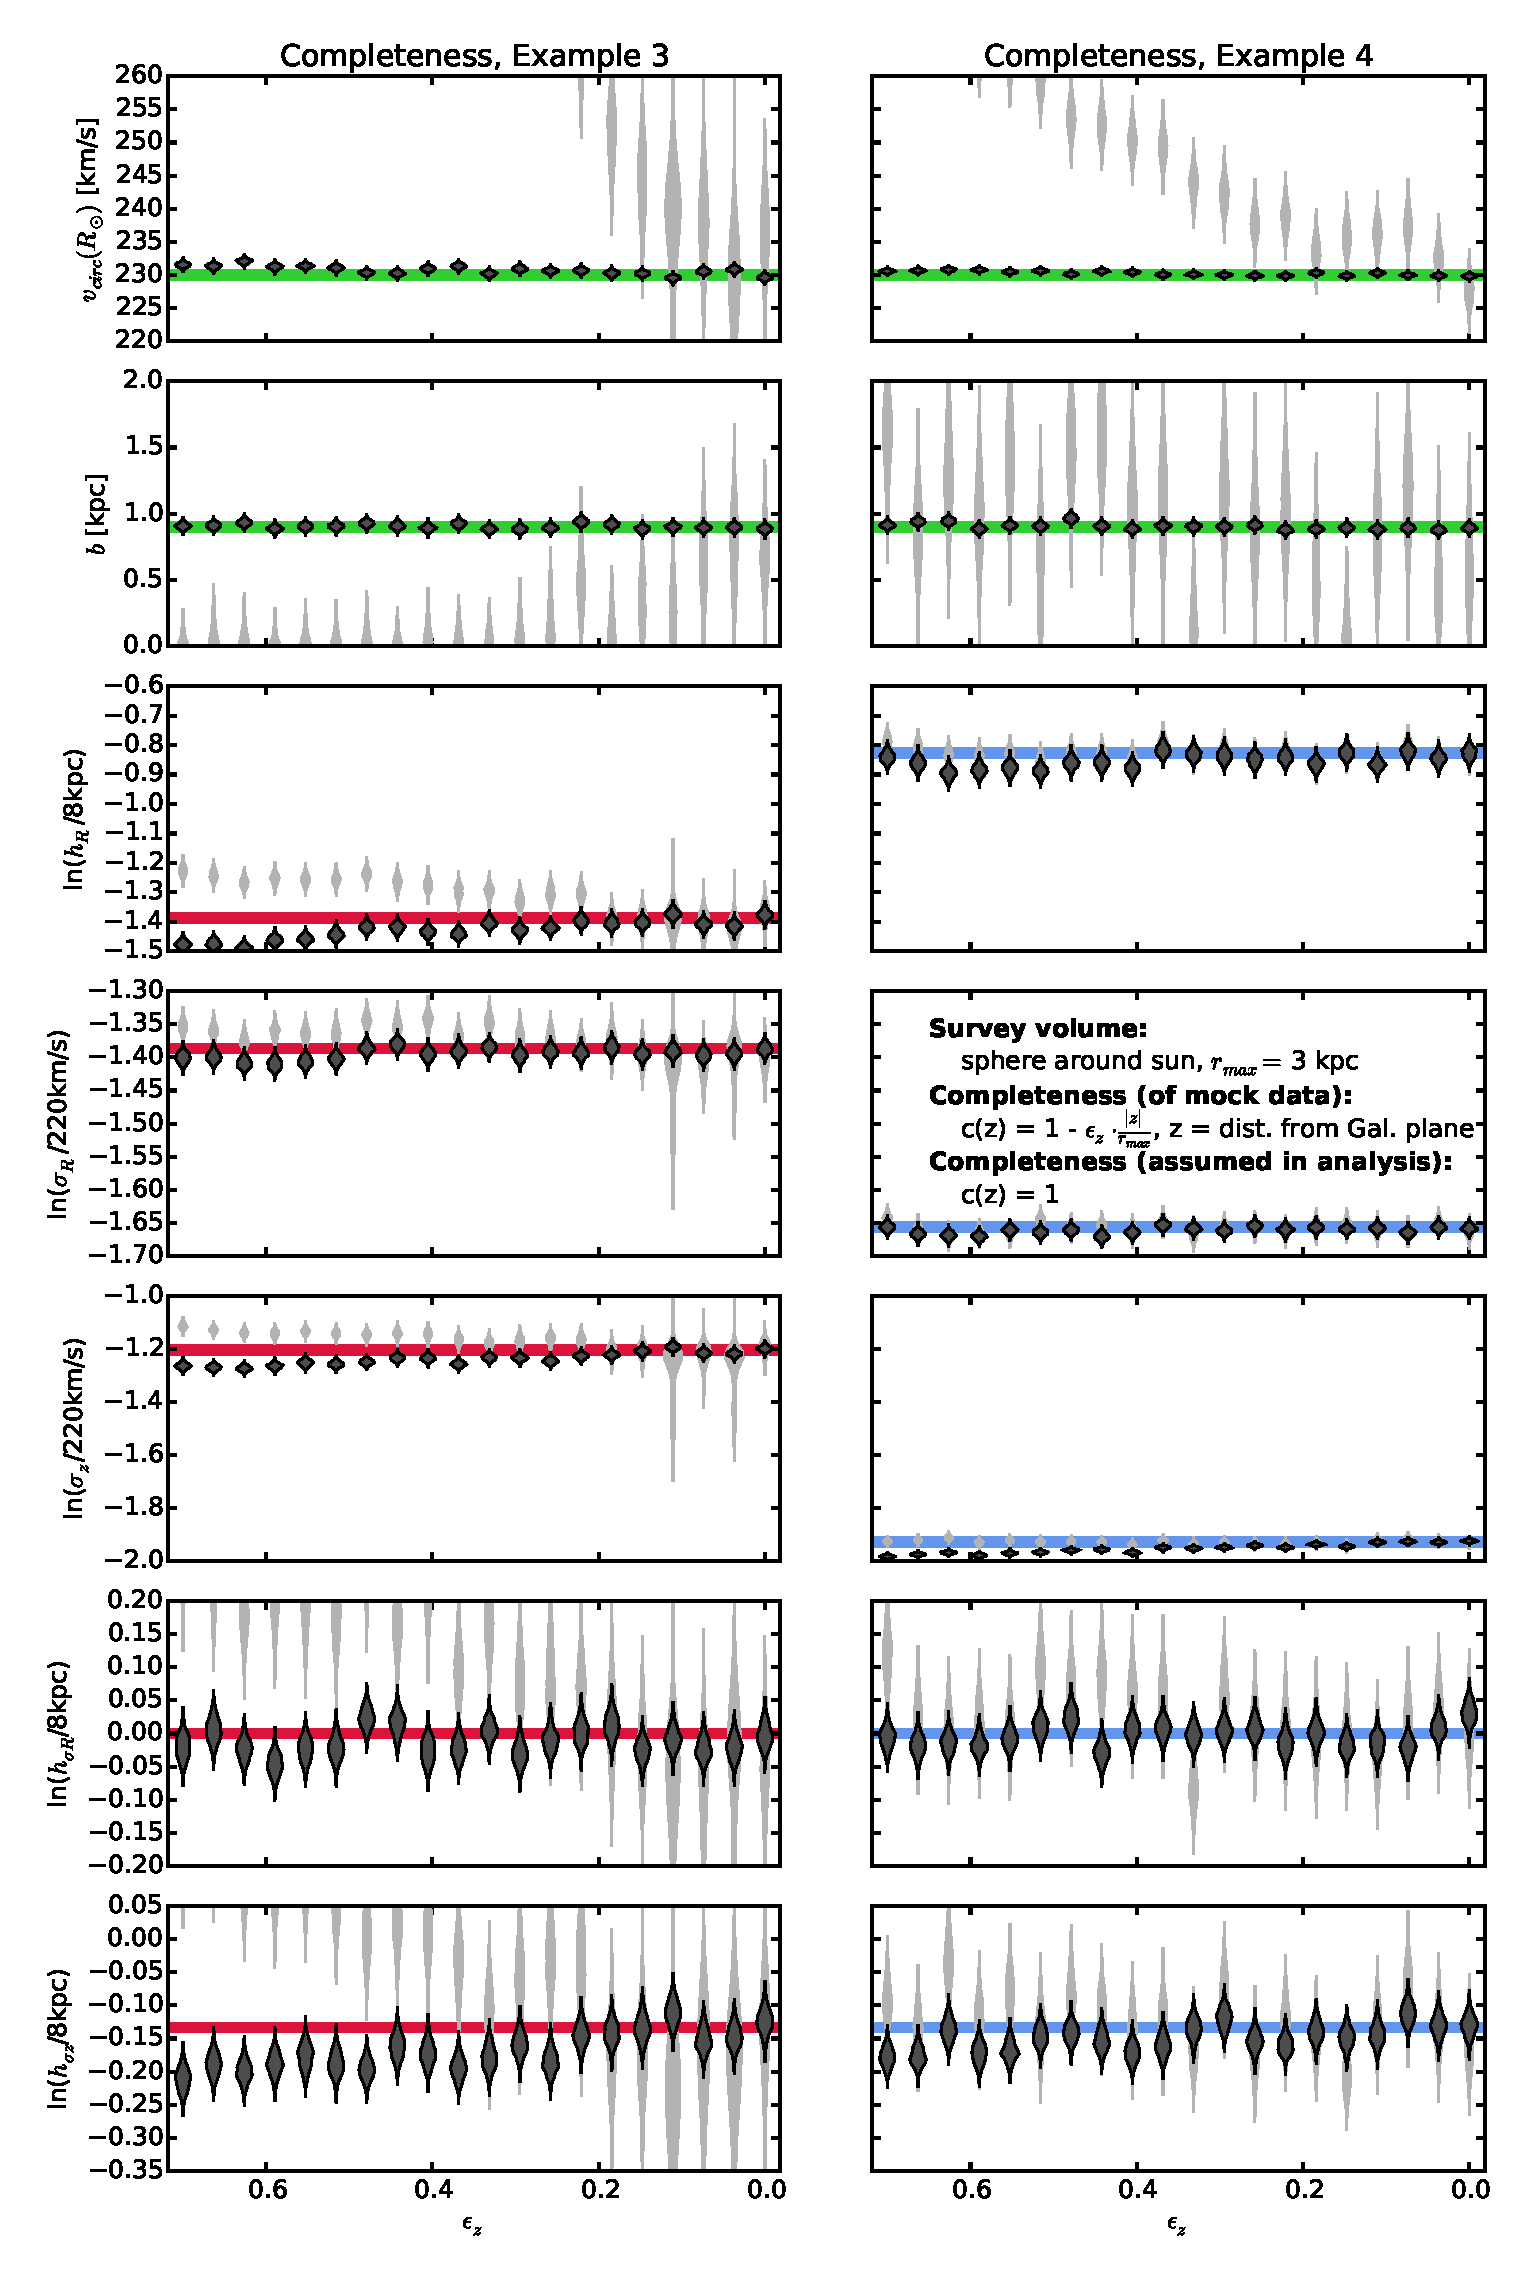
\includegraphics[width=0.8\textwidth]{figs/isoSphFlexIncompZ_violins.eps}
\caption{(Caption on next page.)}
\end{figure*}


\addtocounter{figure}{-1}
\begin{figure*} [t!]
\caption{Influence of wrong assumptions about the incompleteness parallel to the Galactic plane of the data on the parameter reocovery with \RM. Each mock data set was created having different incompleteness parameters $\epsilon_z$ (shown on the $x$-axis and illustrated in Fig. \ref{fig:isoSphFlexIncompZ_mockdata}) and the model parameters are given as test \textcircled{5}, Example 2, in Table \ref{tbl:tests}. The analysis however didn't know about the incompleteness and assumed that all data sets had constant completeness within the survey volume ($\epsilon_z = 0$). The marginalized likelihoods from the fits are shown as violins. The green lines mark the true potential parameters ("Iso-Pot") and the red and blue lines the true qDF parameters ("hot" \MAP in red and "cool" \MAP in blue), which we tried to recover. The \RM method seems to be robust against small to intermediate deviations between the true and the assumed vertical data incompleteness, as well as the radial incompleteness in Fig. \ref{fig:isoSphFlexIncompZ_violins}.} 
\label{fig:isoSphFlexIncompZ_violins}
\end{figure*}

\begin{figure*}
\plotone{figs/isoSphFlexIncomp_marginal_violins.eps}
\caption{Influence of wrong assumptions about radial and vertical incompleteness on the parameter recovery, when \emph{not} including information about the tangential velocities in the analysis. The mock data sets are the same as in Fig. \ref{fig:isoSphFlexIncompR_violins} and \ref{fig:isoSphFlexIncompZ_violins}, but this time we did not include the data coordinates $v_T$ in the analysis and therefore marginalized the likelihood over $v_T$ instead (see \S\ref{sec:incompZ}). This demonstrates that a lot of information about the potential is actually stored in the rotation curve, i.e. $v_T(R)$, which is not affected by removing stars from the data set. But even if we do not include $v_T$ we can still recover the potential within the errors, at least for small ($\epsilon_z \lesssim 10\%$).} 
\label{fig:isoSphFlexIncomp_marginal_violins}
\end{figure*}
}
\end{appendix}

\section{Questions that haven't been covered so far:}

\begin{itemize}
\item What limits the overall code speed?
\item What happens, when the errors are not uniform?
\item What if errors in distance matter for selection?
\item Deviations from axisymmetry: Take numerical simulations.
\end{itemize}

\paragraph{Stuff that needs to be further examined about the robustness against data incompleteness:}
\begin{itemize}
\item[[TO DO]] Maybe instead of decreasing completeness with height above the plane, a completeness
that INcreases with height above the plan, to model e.g. obscuration due to dust.
\item[[TO DO]] Make similar test as isoSphFlexIncompR, but with KKS potential, to test, if this
robustness is a special case for the isochrone potential.
\end{itemize}

\paragraph{General Stuff}
\begin{itemize}
\item[[TO DO:]] Rename everywhere $N_\text{sigma}$ to $n_\text{interval}$ or something like this.
\item[[TO DO:]] Look up what McMillan \& Binney 2013 have to say about the numerical accuracy of the normalisation. Sanders \& Binney (2015) are quoting them on that matter.
\item[[TO DO:]] Consistent capitals in section titles.
\item[[TO DO:]] Make consistent: use of $\sigma_{R,0}$ and $\sigma_R$ as profile or dispersion at sun.
\item[[TO DO:]] Make consistent $h_{\sigma_R}$ --> $h_{\sigma,R}$
\item[[TO DO:]] Make consistent $M$ --> \pmodel
\item[[TO DO:]] Make consistent MAP --> \MAP
\item[[TO DO:]] Make consistent number of stars $N$ --> $N_\text{sample}$, introduce somewhere
\item[[TO DO:]]  introduce \pdf somewhere
\end{itemize}

%=====================================================

%15. May 2015 --> Meet with HW to write
%
%* just explain what the best solution in analysis section is, don't explain too much about other (worse) techniques
%* Numerical accuracy plot is a result
%* 20,000 stars --> much larger than current sample sizes (200 stars), but forecasting to larger sample sizes with Gaia (?)
%* Fig. 3,4,5 --> Behaviour in the limit of large samples
%* Change order of sections according to order in Results section intro
%* mention in introduction that we do not investigate axisymmetry
%* limit of lousy data --> model assumptions are not limiting. very good data --> model assumptions are limiting. Bovy & Rix: 150 stars per MAP. When we get larger samples sizes, the modelling will be limited by the model assumptions.
%* rename model parameters $M$ into $p_M$
%* mock data in action space plot --> in mock data section
%* accuracy plot --> in "Numerical accuracy of the likelihood calculation" section
%* in section on numerical accuracy erwähnen, dass wir in the limit of many stars aufpassen müssen, dass wir die normalisierung genau genug berechnen.
%* Macro fuer MAP schreiben: In Kapitälchen, damit klar ist, dass das ein Akronym ist
%* Citation korrigieren: bo13 --> bov13
%* Check how many stars were typically in a Bovy&Rix13 MAP
%* Triangle plot --> I talk about likelihood, but it is a pdf!
%* Priors: We want parameter estimates that alre tight enough, such that it does not matter, if we had assumed a flat or a logarithmically flat prior
%* Introduce somewhere the 20,000 stars 
%* if the priors are sufficiently flat, likelihood and pdf are the same.
%* rename $N_j$ into $N_sample$
%* change <_ 1 in eq. 5 to <_ 1/N_sample
%* Mach einheitlich: width of pdf, likelihood, Standard error --> $\sigma_p$ ???
%* schwarze punkte in (un)-bias CLT plot: call "pdf expectation value"
%* triangle plot: potential-potential, qdf-qdf und potential-qdf panels in unterschiedlichen Farbschemen.
%* Error on the width of the likelihood scales also with 1/sqrt(N) or sqrt(N-1) --> nicht in sqrtN figure einzeichnen, weil mein scatter größer ist. Neu berechnen?
%* Latex Tipp: ~ ist ein halber Abstand.
%* TO DO: Test, if characteristic errors indeed smaller than disp --> negligible
%* obsvolumetest: orange volume eine breite weiter nach oben, also leicht oberhalb der plane.
%* replace "cf." with "see" everywhere
%* Latex Tipp: Häufige Bennenungen als Befehle definieren. Lässt sich nachträglich leichter ändern.
%* Check that CLT plot and volumetestplot have both 20,000 stars
%* epsilon ist was kleines, sollte also nicht 100% sein (incompleteness ...)

%26. June 2015 --> Meet with HW to write
%* Make consistent: fig. --> Fig., table --> Table, eq. --> Eq.
%* change examples 1-4 to examples 1a/b and 2a/b
%* reference always in text that exact model parameters are mentioned in figure caption
}








[TO DO: Check if all references are actually used in paper. ???]

\begin{thebibliography}{}
\bibitem[Batsleer \& Dejonghe(1994)]{bat94} [TO DO]
\bibitem[Binney \& McMillan(2011)]{bin11} Binney, J. J., \& McMillan, P. 2011, \mnras, 413, 1889
\bibitem[Binney(2012)]{bin12} Binney, J. J. 2012, \mnras, 426, 1324
\bibitem[Bovy et al.(2012b)]{bov12b} Bovy, J., Rix, H.-W., \& Hogg, D. W. 2012b, \apj, 751, 131
\bibitem[Bovy et al.(2012c)]{bov12c} Bovy, J., Rix, H.-W., Hogg, D. W. et al., 2012c, \apj, 755,115
\bibitem[Bovy et al.(2012d)]{bov12d} Bovy, J., Rix, H.-W., Liu, C. et al., 2012d, \apj, 753, 148
\bibitem[Bovy \& Rix(2013)]{bov13}  Bovy, J., \& Rix, H.-W. 2003, \apj, 779, 115
\bibitem[Piffl et al.(2014)]{pif14} Piffl, T., Binney, J., \& McMillan, P. J. et al., 2014, \mnras, 455, 3133
\bibitem[Steinmetz et al.(2006)]{ste06} Steinmetz, M. et al., 2006, \aj, 132, 1645
\bibitem[Ting et al.(2013)]{tin13} Ting, Y.-S., Rix, H.-W., Bovy, J., \& van de Ven, G. 2013, \mnras, 434, 652
\bibitem[Binney \& Tremaine(2008)]{bin08} Binney, J., \& Tremaine, S. 2008, [TO DO: Galactic Dynamics???]
\bibitem[Sanders \& Binney(2015)]{san15} [TO DO] Sanders \& Binney (2015) Extended distribution functions for our Galaxy
\bibitem[Bovy(2015)]{bov15} [TO DO] Bovy (2015) Galpy paper
\end{thebibliography}



\end{document}

